\documentclass[journal]{vgtc}                     % final (journal style)
%\documentclass[journal,hideappendix]{vgtc}        % final (journal style) without appendices
% \documentclass[review,journal]{vgtc}              % review (journal style)
%\documentclass[review,journal,hideappendix]{vgtc} % review (journal style)
%\documentclass[widereview]{vgtc}                  % wide-spaced review
%\documentclass[preprint,journal]{vgtc}            % preprint (journal style)

\usepackage{tabularray}

%\usepackage[english]{babel}
%\usepackage[colorlinks=true, allcolors=blue]{hyperref}
%% Uncomment one of the lines above depending on where your paper is
%% in the conference process. ``review'' and ``widereview'' are for review
%% submission, ``preprint'' is for pre-publication in an open access repository,
%% and the final version doesn't use a specific qualifier.

%% If you are submitting a paper to a conference for review with a double
%% blind reviewing process, please use one of the ``review'' options and replace the value ``0'' below with your
%% OnlineID. Otherwise, you may safely leave it at ``0''.
%\usepackage{hyperref}

\onlineid{1314}

%\renewcommand*{\sectionautorefname}{Section}
%\renewcommand*{\subsectionautorefname}{Section}
%\renewcommand*{\subsubsectionautorefname}{Section}
%% In preprint mode you may define your own headline. If not, the default IEEE copyright message will appear in preprint mode.
%\preprinttext{To appear in IEEE Transactions on Visualization and Computer Graphics.}

%% In preprint mode, this adds a link to the version of the paper on IEEEXplore
%% Uncomment this line when you produce a preprint version of the article 
%% after the article receives a DOI for the paper from IEEE
%\ieeedoi{xx.xxxx/TVCG.201x.xxxxxxx}

%% declare the category of your paper, only shown in review mode
\vgtccategory{Research}

%% please declare the paper type of your paper to help reviewers, only shown in review mode
%% choices:
%% * algorithm/technique
%% * application/design study
%% * evaluation
%% * system
%% * theory/model
%\vgtcpapertype{please specify}
\vgtcpapertype{application/design study}

% Add command
\newcommand{\qevis}{{\sf QEVIS}}
%\newcommand{\hive}{{\sf Apache Hive}}
\newcommand{\hive}{{Apache Hive}}
\newcommand{\vtitle}[1]{{\textit{#1}}}

\newcommand{\stitle}[1]{\vspace*{0.1em}\noindent{\bf #1.\/}}
\newcommand{\sstitle}[1]{\vspace*{0.2em}\noindent{\bf #1:\/}}
\newcommand{\ssstitle}[1]{\vspace*{0.2em}\noindent{\it #1\/}}
\newcommand{\sxtitle}[1]{\vspace*{0.2em}\noindent{\bf #1\/}}
\newcommand{\sssstitle}[1]{\vspace*{0.1em}\noindent{\bf #1:\/}}

\newcommand{\squishlist}{
	\begin{list}{$\bullet$}
		{ \setlength{\itemsep}{0pt}
			\setlength{\parsep}{1pt}
			\setlength{\topsep}{1pt}
			\setlength{\partopsep}{0pt}
			\setlength{\leftmargin}{1.6em}
			\setlength{\labelwidth}{1em}
			\setlength{\labelsep}{0.6em}
		}
	}
	\newcommand{\squishend}{
	\end{list}
}

\newcommand{\qm}[1]{{\color{black}{#1}}}
\newcommand{\nv}[1]{{\color{red}{#1}}}


\newcommand{\aps}{{\mathsf{APS}}}
\newcommand{\ads}{{\mathsf{ADS}}}


\usepackage{hyperref}
%\usepackage[english]{babel}
%\addto\extrasenglish{
%	\renewcommand{\sectionautorefname}{AutoRefSection}
%	\let\subsectionautorefname\sectionautorefname
%	\let\subsubsectionautorefname\sectionautorefname
%}

%\renewcommand{\thesubsubsection}{\thesection.\arabic{subsubsection}}
\renewcommand*{\sectionautorefname}{Section}
\renewcommand*{\subsectionautorefname}{Section}
\renewcommand*{\subsubsectionautorefname}{Section}


%\renewcommand*{\thesection}{section}
%\renewcommand*{\thesubsection}{subsection}
%\renewcommand*{\thesubsubsection}{subsubsection}
%% Paper title.
\title{\qevis: Multi-grained Visualization of Distributed Query Execution}

%% Author ORCID IDs should be specified using \authororcid like below inside
%% of the \author command. ORCID IDs can be registered at https://orcid.org/.
%% Include only the 16-digit dashed ID.
% \author{%
%   \authororcid{Josiah S.\ Carberry}{0000-0002-1825-0097},
%   Ed Grimley, and 
%   Martha Stewart
% }

\author{%
  Qiaomu Shen, Zhengxin You, Xiao Yan, Chaozu Zhang, Ke Xu, Dan Zeng, Jianbin Qin, Bo Tang
}

% \authorfooter{
%   %% insert punctuation at end of each item
%   \item
%   	Josiah Carberry is with Brown University.
%   	E-mail: jcarberry@example.com
%   \item
%   	Ed Grimley is with Grimley Widgets, Inc.
%   	E-mail: ed.grimley@example.com.

%   \item Martha Stewart is with Martha Stewart Enterprises at Microsoft
%   Research.
%   	E-mail: martha.stewart@example.com.
% }

\authorfooter{
	%% insert punctuation at end of each item
        \item
	Qiaomu Shen is with Research Institute of Trustworthy Autonomous Systems, Southern University of Science and Technology. 
	E-mail: shenqm@sustech.edu.cn.
	\item
	Zhengxin You, Xiao Yan, Chaozu Zhang, Dan Zeng and Bo Tang are with Department of Computer Science and Engineering, Southern University of Science and Technology. 
	E-mail: {\{12250078@mail.,yanx@, 12132372@mail., zengd@, tangb3@\}sustech.edu.cn}.
	\item
	Ke Xu is with Huawei Technologies Co., Ltd.
	E-mail: xuke81@huawei.com.
	\item
	Jianbin Qin is with Shenzhen Institute of Computing Sciences, Shenzhen University.
	E-mail: qinjianbin@szu.edu.cn.
	\item
	Jianbin Qin and Bo Tang are the corresponding authors.
}

%% Abstract section.
%Apache \hive{} has been widely used in many organizations for large-scale data analytics applications, and analyzing and accelerating its query execution process are daily routines for engineers and developers.
%However, existing visualization tools for query execution are insufficient because (i) most of them (if not all) do not support fine-grained (i.e., task level) exploratory analysis, which is essential for understanding query performance, 
%and (ii) they do not provide proper linkages between system status and query execution, which makes it difficult to identify the root causes of abnormal behaviors.
%
%Motivated by these limitations, we propose a visual analytics system \qevis{}, which supports visual exploration of query execution at multiple levels of granularity in Apache \hive{}.
%Specifically, we first devise an efficient query plan layout algorithm to visualize the high-level execution progress compactly and clearly.
%We then propose two novel scoring methods to summarize the anomaly degrees of the jobs and machines during query execution, and visualize them effectively.
%Next, we devise a scatter plot-based \vtitle{task view} to show the details of query execution progress.
%Moreover, we equip $\qevis$ with a suite of auxiliary views and interaction methods to support easy and effective cross-view exploration.
%$\qevis$ has been used in the production environment of our industry partner Huawei Cloud, and 
%we present three use cases from real-world applications to demonstrate the effectiveness of $\qevis$.
%$\qevis$ is open-source at \url{https://github.com/vis4db/qevis}.
%the details of query execution progress
\abstract{Distributed query processing systems such as \hive{} and Spark are prevalent in organizations that require large-scale data analytics. Analyzing and understanding the query execution process of these systems are daily routines for engineers and crucial for identifying performance problems, optimizing system configurations, and rectifying errors. 
However, existing visualization tools for distributed query execution are insufficient because (i) most of them (if not all) do not provide fine-grained visualization (i.e., the atomic task level), 
%which is essential for understanding query performance and reasoning execution problems, 
\qm{which can be crucial for understanding query performance and reasoning about the underlying execution anomalies}, 
and (ii) they do not support proper linkages between system status and query execution, which makes it difficult to identify the causes of execution problems.
To tackle these limitations, we propose \qevis{}, which visualizes distributed query execution process with multiple views that focus on different granularities and complement each other.
Specifically, we first devise a query logical plan layout algorithm to visualize the overall query execution progress compactly and clearly.
We then propose two novel scoring methods to summarize the anomaly degrees of the jobs and machines during query execution, and visualize the anomaly scores intuitively, which allow users to easily identify the components that \qm{are worth paying attention to}.
Moreover, we devise a scatter plot-based \vtitle{task view} to show a massive number of atomic tasks, where task distribution patterns are informative for execution problems.
We also equip \qevis{} with a suite of auxiliary views and interaction methods to support easy and effective cross-view exploration, which makes it convenient to track the causes of execution problems.
\qevis{} has been used in the production environment of our industry partner, and 
we present three use cases from real-world applications to demonstrate its effectiveness.
\qevis{} is open-source at \url{https://github.com/vis4db/qevis}.
%to track the causes of execution problems
}

%% Keywords that describe your work. Will show as 'Index Terms' in journal
%% please capitalize first letter and insert punctuation after last keyword
\keywords{visual analytics system, distributed query execution, performance analysis}

%% A teaser figure can be included as follows
\teaser{
  \centering
  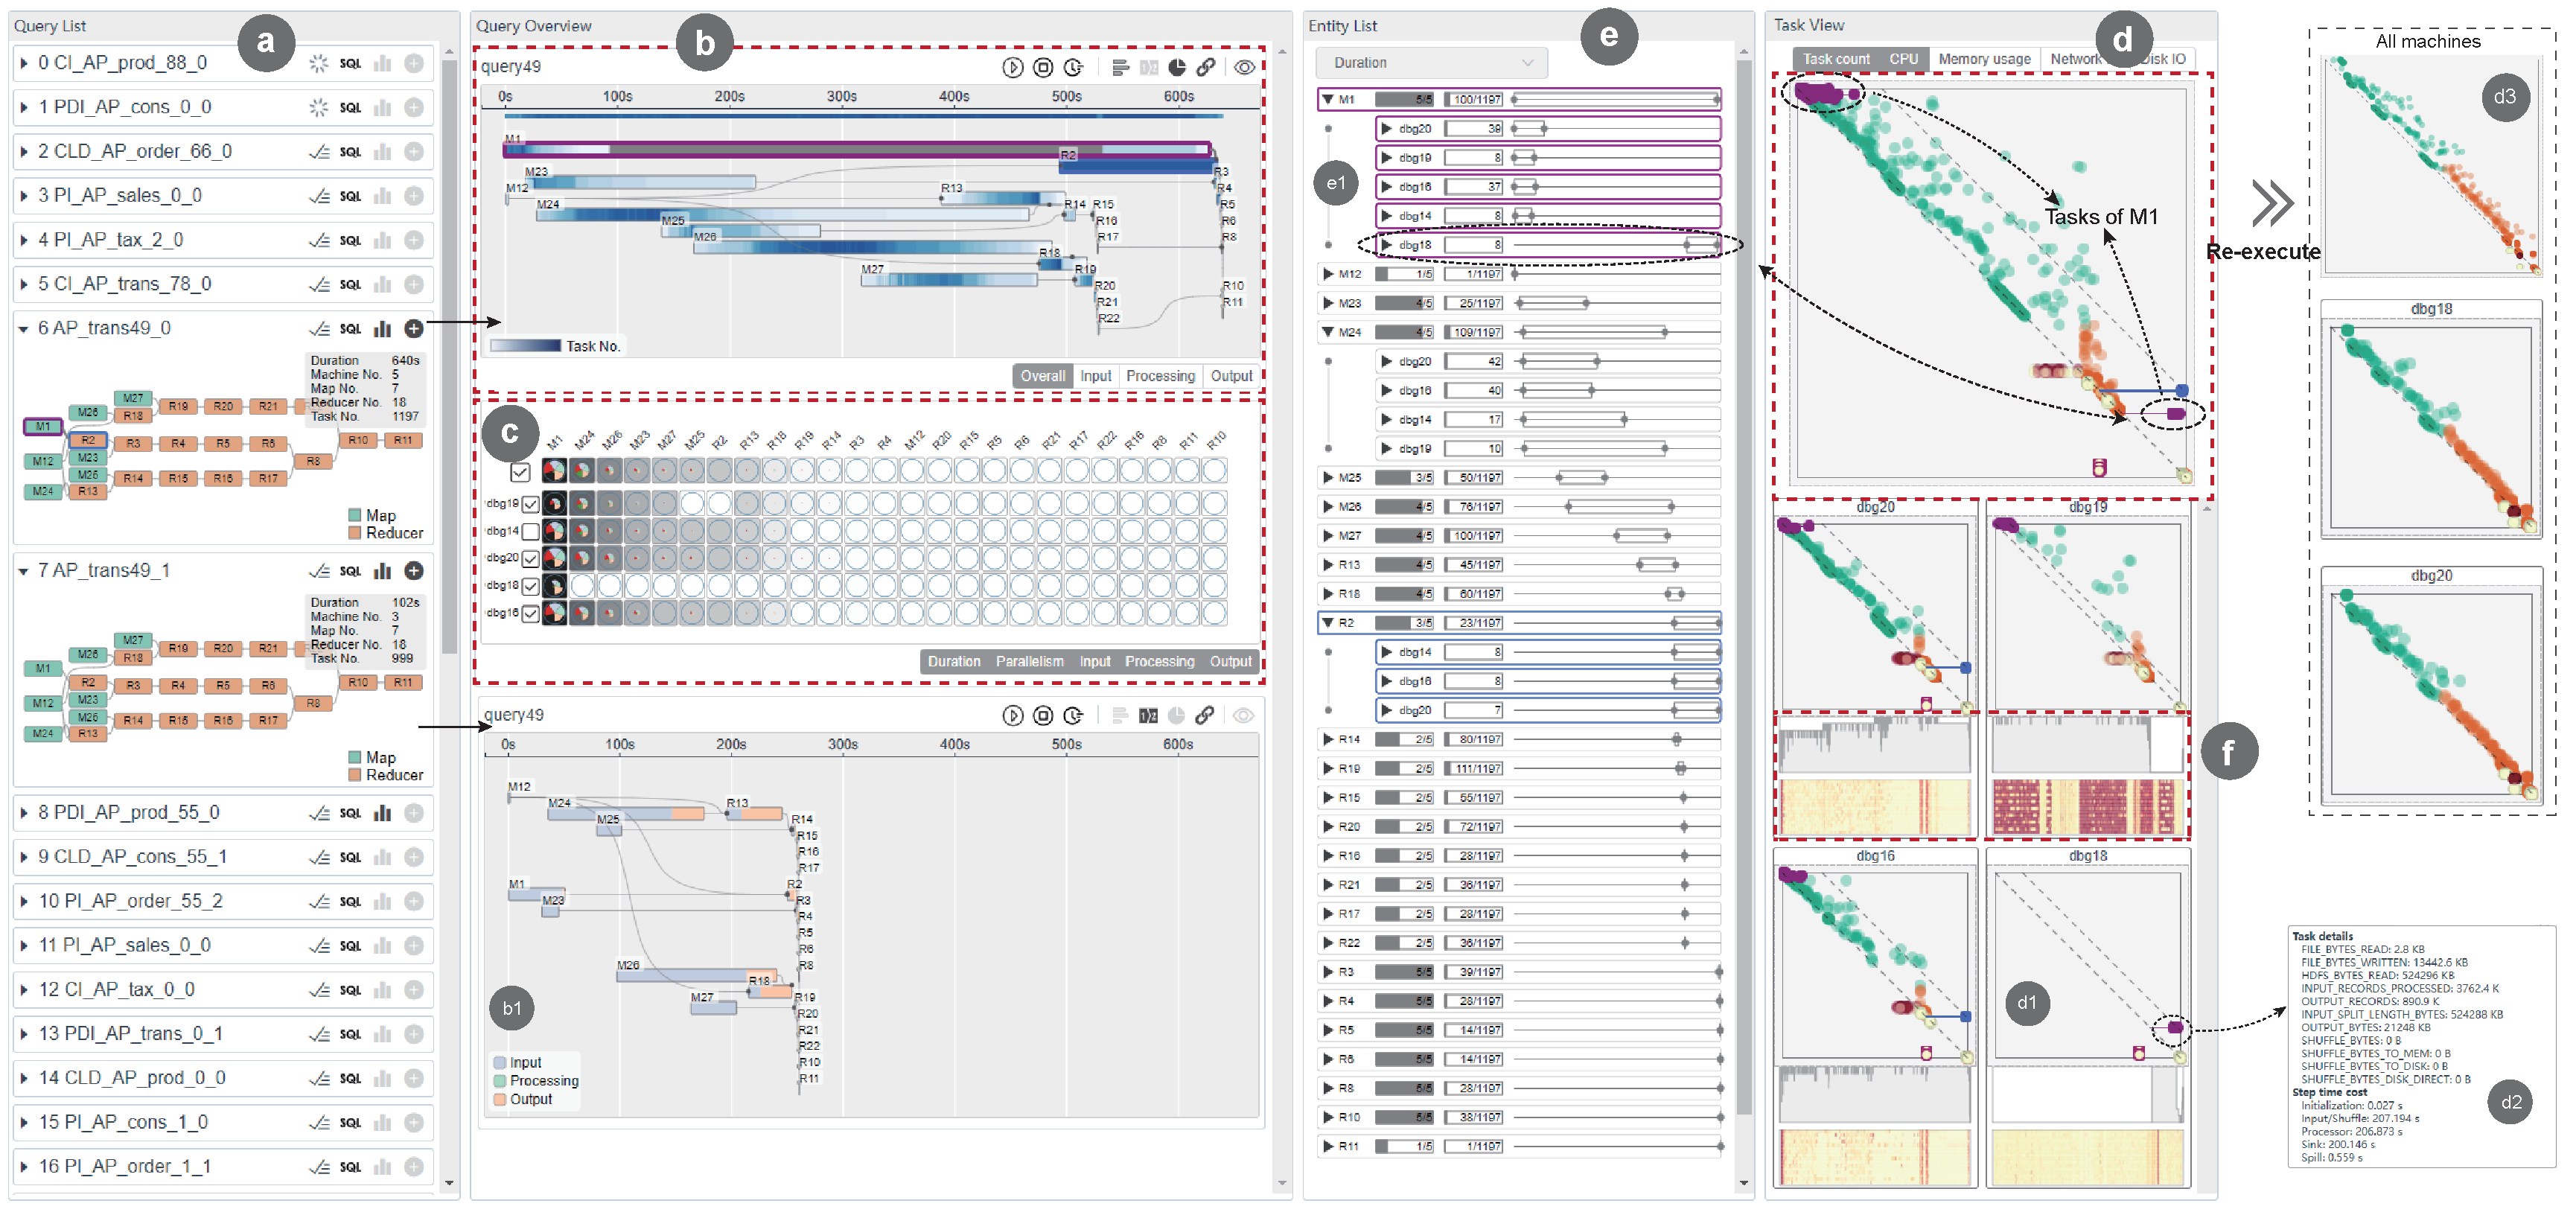
\includegraphics[width=0.92\linewidth]{figures/teaser/teaserSDS_pdf.pdf}
	\caption{
%The UI of \qevis{}, which visualizes distributed query execution with multiple complementing views. (a) \vtitle{Query list} displays all queries and allows to select a query for analysis. (b) \vtitle{Job view} depicts the execution progress of the jobs in a query and their dependencies for an overview of query execution. (c) \vtitle{Performance matrix} shows the anomaly degrees of the jobs and machines to quickly identify execution anomalies. To \qm{reason about} the anomalies: (d) \vtitle{Task view} plots the distribution of the atomic tasks; (e) \vtitle{Entity list} reports detailed task execution statistics; (f) \vtitle{Profiling view} presents hardware status. These views are well-coordinated for exploration.
The UI of \qevis{} consists of multiple complementary views. (a) \vtitle{Query list} displays all queries and enables query selection for analysis. (b) \vtitle{Job view} depicts the execution progress of the jobs in a query and their dependencies for an overview of query execution. (c) \vtitle{Performance matrix} reveals anomaly degrees of jobs and machines, facilitating the rapid identification of execution anomalies. To \qm{reason about} the anomalies: (d) \vtitle{task view} plots the distribution of atomic tasks. (e) \vtitle{entity list} reports detailed task execution statistics. (f)  \vtitle{Profiling view} presents hardware status. These coordinated views collectively enhance the exploration of query execution dynamics.
	}
  \label{fig:teaser}
}

%
%\begin{figure*}
%	\centering
%	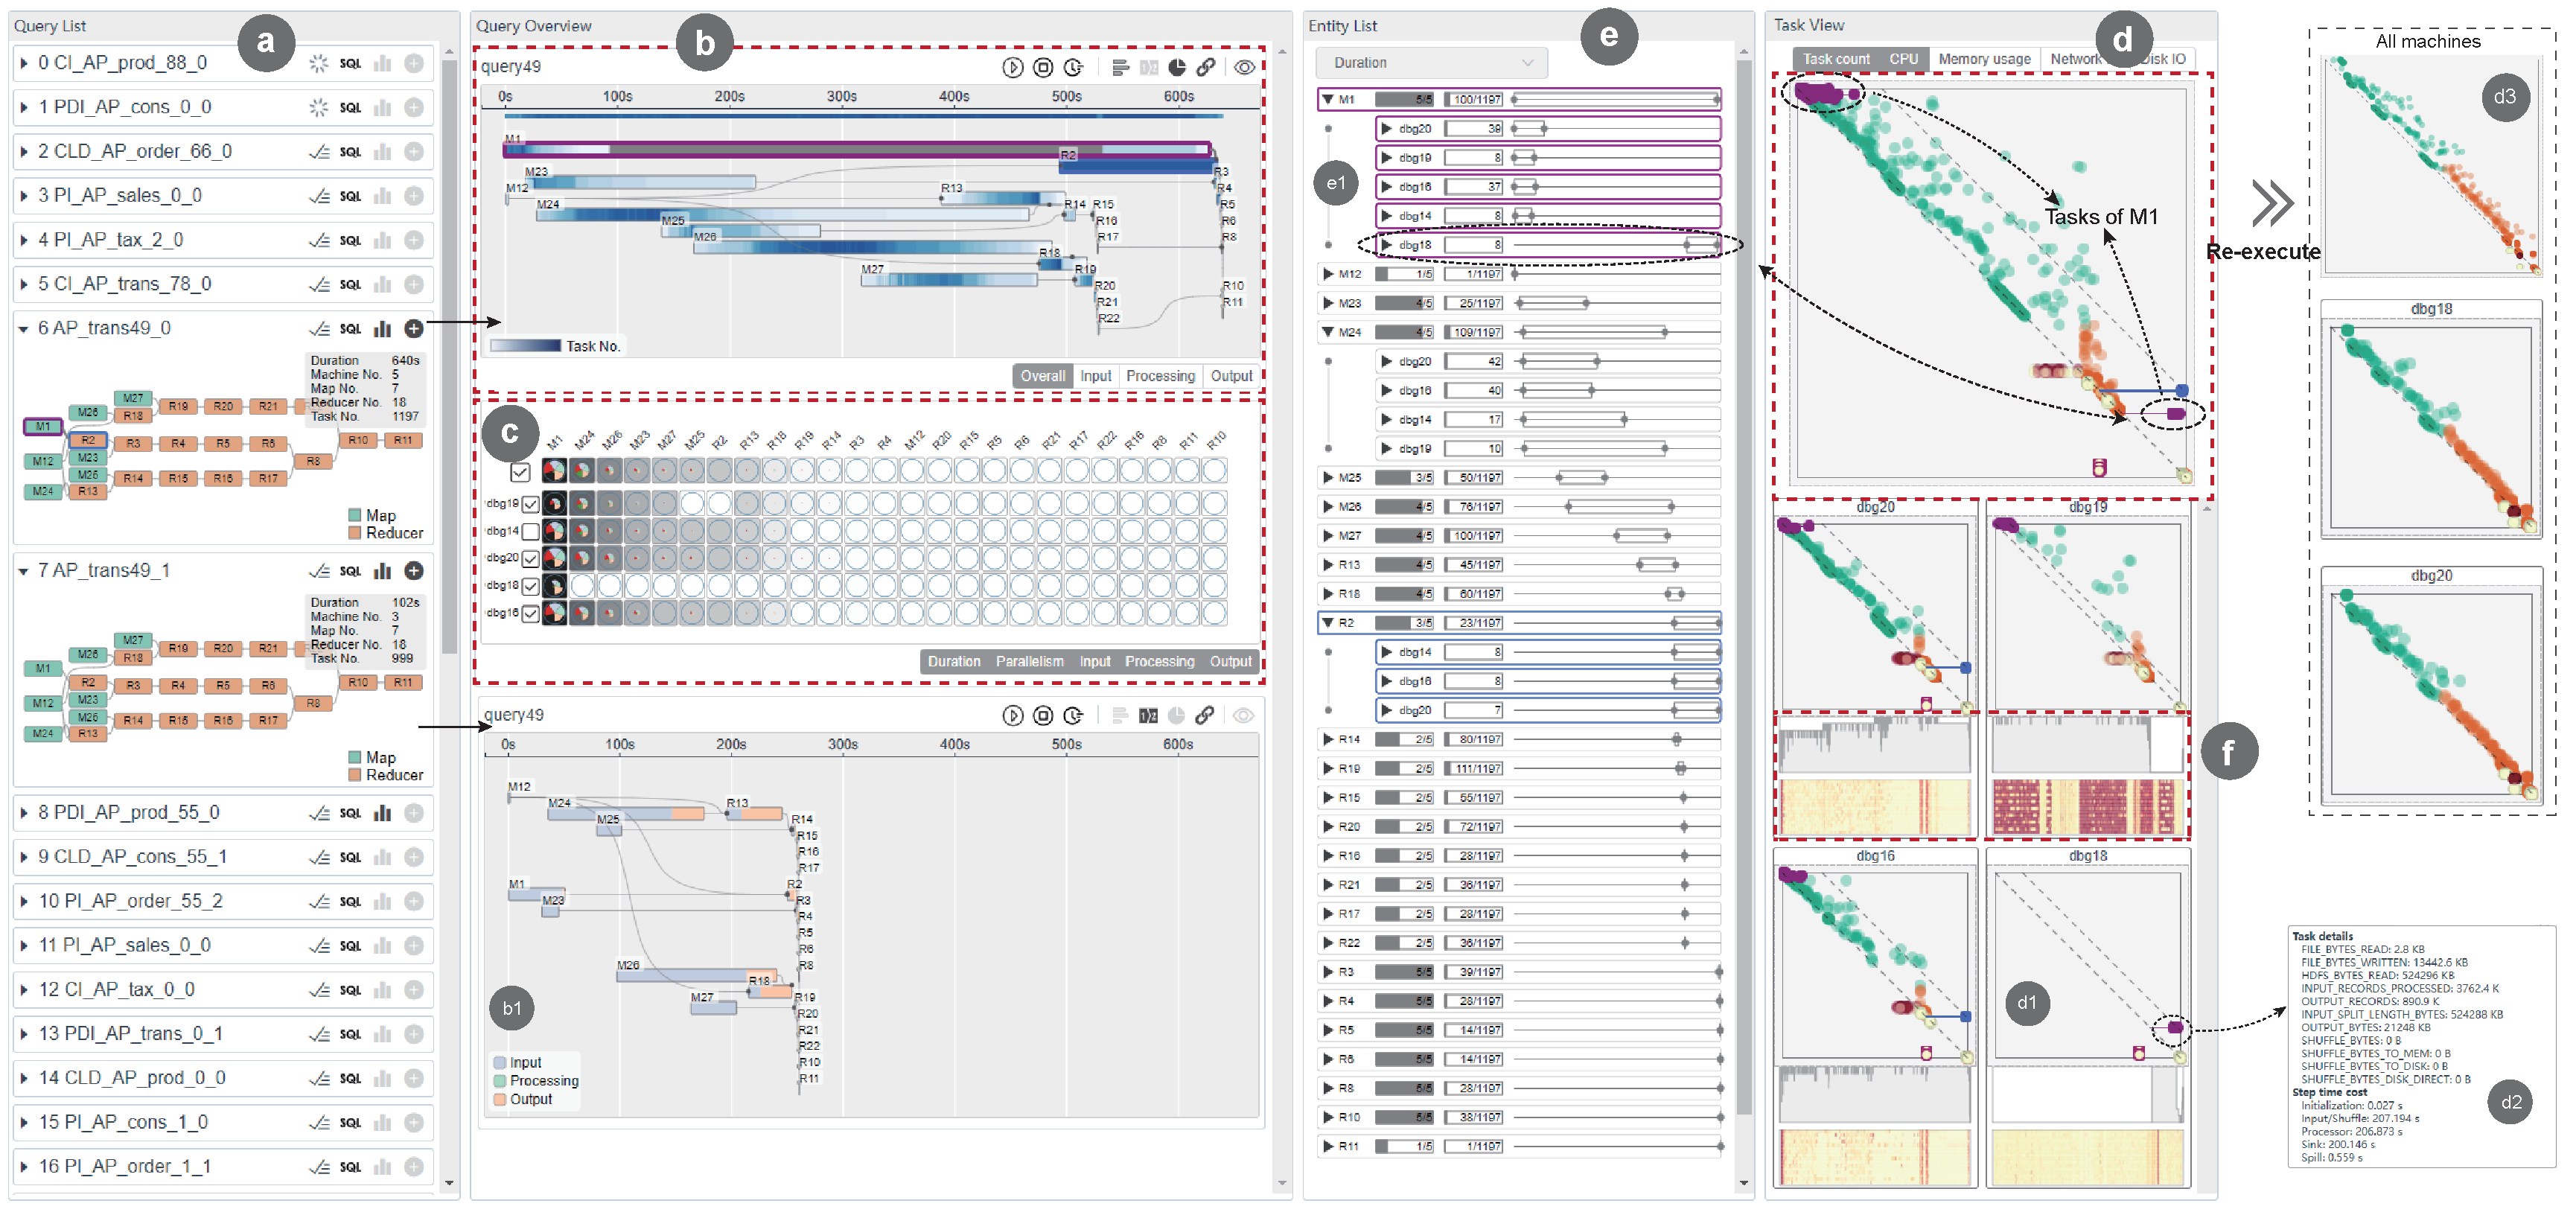
\includegraphics[width=0.98\linewidth]{figures/teaser/teaserSDS_pdf.pdf}
%	\vspace{-3mm}
%	\caption{User interface of \qevis{}. (a) \vtitle{Query list} displays all analysis queries. (b) \vtitle{Job view} depicts the query execution progress. (c) \vtitle{Performance matrix} shows the anomaly degree. (d) \vtitle{Task view} assists task analysis. (e) \vtitle{Entity list} presents task execution statistics. (f) \vtitle{Profiling view} summarizes hardware status.}
%	\label{fig:teaser}
%	\vspace{-3mm}
%\end{figure*}
%% Uncomment below to disable the manuscript note
%\renewcommand{\manuscriptnotetxt}{}

%% Copyright space is enabled by default as required by guidelines.
%% It is disabled by the 'review' option or via the following command:
%\nocopyrightspace


%%%%%%%%%%%%%%%%%%%%%%%%%%%%%%%%%%%%%%%%%%%%%%%%%%%%%%%%%%%%%%%%
%%%%%%%%%%%%%%%%%%%%%% LOAD PACKAGES %%%%%%%%%%%%%%%%%%%%%%%%%%%
%%%%%%%%%%%%%%%%%%%%%%%%%%%%%%%%%%%%%%%%%%%%%%%%%%%%%%%%%%%%%%%%

%% Tell graphicx where to find files for figures when calling \includegraphics.
%% Note that due to the \DeclareGraphicsExtensions{} call it is no longer necessary
%% to provide the the path and extension of a graphics file:
%% \includegraphics{diamondrule} is completely sufficient.
\graphicspath{{figs/}{figures/}{pictures/}{images/}{./}} % where to search for the images

%% Only used in the template examples. You can remove these lines.
\usepackage{tabu}                      % only used for the table example
\usepackage{booktabs}                  % only used for the table example
\usepackage{lipsum}                    % used to generate placeholder text
\usepackage{mwe}                       % used to generate placeholder figures

%% We encourage the use of mathptmx for consistent usage of times font
%% throughout the proceedings. However, if you encounter conflicts
%% with other math-related packages, you may want to disable it.
\usepackage{mathptmx}                  % use matching math font
%
%\addto\extrasenglish { 	
%	\renewcommand{\sectionautorefname}{Section}
%	\let\subsectionautorefname\sectionautorefname
%	\let\subsubsectionautorefname\sectionautorefname 
%}
%\newcommand*{\sectionautorefname}{Section}

\begin{document}

%%%%%%%%%%%%%%%%%%%%%%%%%%%%%%%%%%%%%%%%%%%%%%%%%%%%%%%%%%%%%%%%
%%%%%%%%%%%%%%%%%%%%%% START OF THE PAPER %%%%%%%%%%%%%%%%%%%%%%
%%%%%%%%%%%%%%%%%%%%%%%%%%%%%%%%%%%%%%%%%%%%%%%%%%%%%%%%%%%%%%%%

%% The ``\maketitle'' command must be the first command after the
%% ``\begin{document}'' command. It prepares and prints the title block.
%% the only exception to this rule is the \firstsection command
%\firstsection{Introduction}


\maketitle

\section{Introduction}\label{sec:intro}
Distributed query processing systems such as \hive{}~\cite{thusoo2009hive}, Spark~\cite{spark}, and Flink~\cite{carbone2015apache} support scalable data analytics on many machines~\cite{thusoo2009hive,thusoo2010hive}.
With a SQL-like interface on top of parallel data processing frameworks (e.g., MapReduce~\cite{hadoop} or Tez~\cite{saha2015apache}), these systems enable users to run queries with SQL semantics instead of implementing low-level parallel computing programs.
For engineers and developers working with these systems, analyzing and optimizing distributed query execution are daily routines. 
Frequently asked questions include ``\emph{Where does the query execution time go?}'', ``\emph{What is the performance bottleneck of the executed query?}'', and ``\emph{Why does the query run slower than expected?}''.
Answering these questions requires a comprehensive understanding of the query execution process and thus is challenging even for experienced engineers. 
This is caused by the inherent complexity of distributed query execution, e.g., there are many parallel tasks (i.e., the atomic unit of query execution), and machine status and concurrent programs can influence task execution in subtle ways.

As visualizations allow intuitive interpretation, many visual analytics tools have been developed to assist the understanding of query execution, e.g., Tez UI~\cite{tezui}, Spark UI~\cite{sparkui}, and Dr. Elephant~\cite{elephant}. 
However, our industry partner found that these tools are insufficient in two key aspects.
(i) \textsf{Visualization granularity}: 
most of them tend to focus on providing a coarse-grained visualization of the query execution process (e.g., the job level) but fine-grained visualization at the atomic task level is essential for purposes such as tracking deadlocks and detecting data skew.
(ii) \textsf{Tool usability}: they only provide limited interactions among different views, and thus users have to manually switch among different views and speculate the linkage among the views. The two limitations also make it difficult for users to identify the root causes of abnormal execution behaviors efficiently.


To overcome the limitations, we propose \qevis{}, a visual analytics system that allows an in-depth understanding of distributed query execution process. 
\qevis{} encompasses a suite of coordinated views that complement each other by visualizing query execution at different granularities. 
Specifically, for a given query, the \vtitle{job view} displays the execution process of the Map/Reducer jobs in the query and their dependencies as an overview. A new temporal directed acyclic graph (TDAG) visualization algorithm is proposed to show the \vtitle{job view} compactly and clearly.
Then, novel anomaly scores are designed and visualized in the \vtitle{performance matrix} to help users identify suspicious jobs and machines for analysis. 
Next, the execution status of the atomic tasks is shown in the \vtitle{task view}, where a scatter-plot-based visualization allows users to observe the patterns of the tasks and identify the tasks that are \qm{worth paying attention to}.
We also incorporate a suite of auxiliary views to assist the users to \qm{reason about} the discovered abnormal patterns.
In particular, the \vtitle{entity list} shows the statistics and detailed information of the components in query execution (e.g., job, task, and machine), and the \vtitle{profiling view} is aligned with the \vtitle{task view} to help users associate machine status with task execution.
We implement well-coordinated linkage mechanisms for related items in different views and provide flexible interactions to navigate among the views, which makes interactive visual exploration easy.

\qevis{} has been deployed in the production environment of our industry partner for over six months. The engineers and developers appreciate that \qevis{} helps them gain an intuitive understanding of the query execution process and easily identify the problems in query execution. 
%To demonstrate the effectiveness of \qevis{}, we report three use cases from real-world applications, which show that the multi-grained visualizations provided by \qevis{} can identify diverse and complex causes for abnormal query execution. We also conduct an interview to collect feedback from the users of \qevis{}.  
\qm{\qevis{} is primarily developed for Apache Hive, however, its fundamental architecture and essential design elements (e.g., \vtitle{job view} and \vtitle{task view}) exhibit broad adaptability. 
	They can be widely adapted to other distributed systems, such as Spark and Flink, that utilize Directed Acyclic Graph (DAG) as their computational abstraction.
}

In particular, we make the following contributions:
\squishlist 
\item \stitle{Multi-grained visualization framework for query execution} 
%By interacting with our industry partner and surveying related work, 
We summarize comprehensive design requirements for the visual analysis of query execution and propose a visualization framework where multiple views complement each other by visualizing query execution at different granularities.  
\item \stitle{New layout algorithm to depict execution overview} We design a novel algorithm to visualize the execution process of the jobs in the query plan and their dependencies.
Compared with existing solutions, our approach optimizes the job layout to display the logic structure clearly while utilizing a smaller rendering space.
\item \stitle{Novel scoring methods to identify execution anomalies} We devise two scoring methods to evaluate the anomaly degree of the tasks spawned by a job. Different from existing scores that consider a specific anomaly, our scores generalize across different anomalies by measuring how far query execution deviates from the ideal case. 
\item \stitle{Scatter-plot-based visualization to show massive tasks} We propose a scatter-plot-based visualization to display the execution details of massive atomic tasks. Compared with existing timeline-based visualizations, our visualization shows the distribution of the massive tasks intuitively and allows users to easily observe important normal/abnormal patterns in query execution.
\item \stitle{Visual analytics system to coordinate multiple views} We build \qevis{} for \hive{}, which properly coordinates the visualizations discussed above. 
%Cross-view linkage and rich interactions are provided to support flexible navigation among the views for problem tracking. 
Cross-view linkage and rich interactions are provided to support flexible navigation among the views.
\squishend



\section{Background}\label{sec:qryprocessing}
To provide background for subsequent discussions, we introduce distributed query execution process using \hive{} as an example.

\begin{figure}[t]
	\centering
	\includegraphics[width=0.40\textwidth]{figures/system/qry_processingvis.pdf}
	\vspace{-3mm}
	\caption{The workflow of distributed query execution in \hive{}}
	\label{fig:qry}
	\vspace{-6mm}
\end{figure}


\autoref{fig:qry} depicts the workflow of query execution in \hive{}.
When a query (e.g., the SQL-like statement in \autoref{fig:qry}(a)) is issued to the system, the query optimizer (e.g., Calcite~\cite{begoli2018apache}) and parallel execution engine (e.g., Tez~\cite{saha2015apache}) optimize and compile the query to a logical execution plan, which is the direct acyclic graph (DAG) of Map/Reducer jobs shown in \autoref{fig:qry}(b).
Each Map or Reducer job in the DAG can be divided into three phases: (1) input, (2) processing, and (3) output.
The input phase loads data from disk or upstream jobs.
The processing phase executes a sequence of SQL operators, for example, the processing phase of Map 1 encompasses three SQL operators: table scan (TS), filter (FIL), and select (SEL).
The output phase generates the output data, which can be the final result or input data for downstream jobs.
The dependencies among the jobs are determined by their input/output relation and modeled by the edges in the DAG.


%, which are the atomic execution units
To run each Map/Reducer job, the execution engine (e.g., Tez) instantiates a set of tasks.
All tasks of a specific Map/Reducer job run the same sequence of operators but work on different data partitions.
For example, the execution engine instantiates three tasks, e.g., $t_{1}[1], t_{1}[2]$, and $t_{1}[3]$ (the gray cells in \autoref{fig:qry}(c)) for job Map 1 in \autoref{fig:qry}(b). 
Each task is scheduled to run on an executor (e.g., container in \hive{}), which is a logical collection of physical resources (e.g., CPU and memory) on one machine in the cluster, by the resource scheduler (e.g., Yarn~\cite{vavilapalli2013apache}).
%Specifically, task is the atomic scheduling unit of a SQL query.
% In addition, different tasks of different jobs can be executed by the same container, i.e., the physical machine.
Task is the atomic unit for execution and scheduling, and the tasks of different jobs can run on the same machine.
For example, as illustrated in \autoref{fig:qry}(c), both $t_{1}[1]$ (a task of Map 1) and $t_{2}[1]$ (a task of Reducer 2) are executed on Machine 1. 

%\qm{
%Based on the workflow shown as \autoref{fig:qry}, existing research works perform the study on visualizing query logic (\autoref{fig:qry}(a)), optimization plan (\autoref{fig:qry}(b)) and execution progress (\autoref{fig:qry}(c)) which will be elaborated in \autoref{sec:relexecution}.
%The research works analyzing the query logic and optimization plan can help analysts diagnose the query logic bugs or optimization bugs. 
%Specifically, \qevis{} is orthogonal to these works and target on diagnosing the query execution trace on the distribution environment. \qevis{} can help to analyze the performance issues caused by hardwares. 
%}

\qm{
%	Building upon the workflow depicted in \autoref{fig:qry}, many research primarily focuses on visualizing query logic (\autoref{fig:qry}(a)) and optimization plans (\autoref{fig:qry}(b)). These research efforts are instrumental in diagnosing query logic bugs or optimization bugs. However, it's important to clarify that \qevis{} is distinct and complementary to these studies. \qevis{} specifically targets the diagnosis of query execution traces (\autoref{fig:qry}(c)) in a distributed environment. \qevis{} is designed to analyze performance issues that may arise due to hardware, providing a unique and necessary perspective in the realm of query execution analysis.
Referring to the workflow in \autoref{fig:qry}, many research work mainly focuses on visualizing query logic (\autoref{fig:qry}(a)) and optimization plans (\autoref{fig:qry}(b)). These studies are very helpful in finding bugs in query logic or optimization. But, it is important to note that \qevis{} is different but complements these studies. \qevis{}  focuses on analyzing query execution traces (\autoref{fig:qry}(c)) in a distributed environment. It is designed to study performance issues that might be caused by the scheduling mechanism, resources, or hardware, etc.
}

%\begin{table*}
%	\caption{The features provided by existing visual analytics tools for query execution and our \qevis{}}
%	\label{tab:approach}
%	\vspace{-2mm}
%	\small
%	\centering
%	\begin{tblr}[		
%		%	caption = {Data description.},
%		%	label={tab:data},
%		%		X[l,m]
%		]{
%			colspec = {X[l,1.7cm]X[l,1.5cm]X[l,1.5cm]X[l,1.6cm]X[l,2.0cm]X[l,2.7cm]X[l,2.5cm]},
%			rowsep = 0.8pt,
%			hlines = {black, },
%			vlines = {black, }, % vlines can not pass through multicolumn cells
%		}
%		\textbf{Tool} & \textbf{Logical plan} & \textbf{Job execution}  & \textbf{Task execution} & \textbf{System profiling} & \textbf{Anomaly score} & \textbf{Cause reasoning}\\
%		Dr. Elephant~\cite{elephant} & No & No & No & No & Specialized heuristic  & Heuristic-based \\
%		TezUI~\cite{tezui} & Yes & Yes & No & No & No & No \\
%		SparkUI~\cite{sparkui} & Yes & Yes & Yes & No & No & No \\
%		DBSherlock~\cite{yoon2016dbsherlock} & No & No & No & Yes & Manual selection & Causality model \\
%		iSQUAD~\cite{ma2020diagnosing} & No & No & No & Yes & Manual selection & Bayesian model \\
%		VQA~\cite{simitsis2014vqa} & Yes & Yes & No & Yes & No & Interactive \\
%		Perfopticon~\cite{moritz2015perfopticon} & Yes & Yes & No & No & No & Interactive \\
%		\qevis{} & \textbf{Yes} & \textbf{Yes} & \textbf{Yes} & \textbf{Yes} & \textbf{General rules} & \textbf{Interactive} 
%	\end{tblr} 
%	\vspace{-3mm}
%\end{table*}


\section{Related Work}\label{sec:rel}
%We compare key related works with our \qevis{} in Table~\ref{tab:approach} and discuss them in greater detail as follows. 
\qm{
%	In this section, we conduct a comprehensive survey of the related work.
In this section, we summarize the techniques that are most related to our work.
}

\subsection{Query Execution Diagnose}
Many systems~\cite{elephant, ma2020diagnosing, yoon2016dbsherlock, teoh2019perfdebug, liu2020fluxinfer, jeyakumar2019explainit, cloudera-manager} design dedicated scores and algorithms to diagnose problems in query execution. 
For example, Dr. Elephant~\cite{elephant} uses configurable rule-based heuristics to evaluate queries executed on Hadoop or Spark and gives suggestions (e.g., increasing virtual memory) to improve query performance. 
PerfXplain~\cite{khoussainova2012perfxplain} offers a query language to express performance queries, along with a decision tree-based algorithm that generates explanations by analyzing a log of query executions.
DBSherlock~\cite{yoon2016dbsherlock} allows users to select a time range that contains anomalies and analyzes the execution statistics and system configurations to explain the anomalies with a causality-based model.
iSQUAD~\cite{ma2020diagnosing} requires users to label abnormal queries and then perform root cause identification using a Bayesian model.
PerfDebug~\cite{teoh2019perfdebug} is a specialized tool designed to analyze computation skew issues. Using data provenance-based techniques, it can automatically identify the records responsible for abnormalities.
We refer interested readers to a comprehensive survey~\cite{gathani2020debugging} on database query debugging. 
These systems work as a black-box that delivers the final diagnosis results (which may be inaccurate) without providing evidence.
Moreover, their scores and algorithms are designed for specific anomalies, e.g., garbage collection time and data skew, but it is difficult to define a complete set of anomalies beforehand in practice and the causes of execution problems can be complex.
% (e.g., the combination of multiple minor anomalies).
Instead of considering a specific anomaly, the anomaly scores in \qevis{} generalize across anomalies by measuring how far query execution deviates from the ideal case. Moreover, \qevis{} provides multiple views and allows to identify the evidence and causes of execution anomalies via interactive exploration, which is more suitable for handling complex execution problems.      

\subsection{Visual Understanding for Query Execution}\label{sec:relexecution}
%V1
%\stitle{Understand query logic}
%For data analytics applications, many queries are obtained by adjusting existing SQL templates and can be complex and difficult to understand. 
%Thus, some work utilize visualizations to help understand query logic.
%Representative methods, such as GraphSQL~\cite{cerullo2007system}, Visual SQL~\cite{jaakkola2003visual} and QueryVis~\cite{leventidis2020queryvis}, utilize node-link diagrams to show the topological structure of query sub-steps. Specifically, GraphSQL~\cite{cerullo2007system} and Visual SQL~\cite{jaakkola2003visual} propose visual query languages that support query visualization and interactive query adjustment.  QueryVis~\cite{leventidis2020queryvis} and STRATISFIMAL LAYOUT~\cite{di2021stratisfimal} propose a visual formalism to provide expressive visual vocabulary encoding for the meaning of SQL queries. They also minimize redundant visual elements to make query logic clear. 
%
%\stitle{Understand logical query execution plan}
%As discussed in \autoref{sec:qryprocessing}, an SQL query is converted into an  execution plan before actual execution, and thus understanding the execution plan is essential for system-level analysis~(e.g., problem diagnosis and improving query optimizer). 
%As execution plans can be modeled as tree or DAG, node-link diagrams based designs are usually used to show their logical structures~\cite{tezui, sparkui, moritz2015perfopticon, battle2016making, simitsis2014vqa}. For instance, Perfopticon~\cite{moritz2015perfopticon} designs a nested node-link diagram to show the hierarchical structure of the execution plan for Myria~\cite{halperin2014demonstration}, a distributed big data system similar to Hive. 
%
%\qm{Understand query logic and execution plan is the key for diagnose the query and optimization logic bugs, which is orthogonal to our target.} 
%

%V2
%\stitle{Understand query statement and logical plan}
%As discussed in \autoref{sec:qryprocessing}, before the execution on the distributed system, an input query is transformed as logical plan.
%Understand the query logic and logical plan is important for users diganose the query logic bugs and optimizations bugs, which has been expo by existing research work. In the real applications, many queries are obtained by adjusting existing SQL templates and can be complex and difficult to understand. Representative methods, such as GraphSQL~\cite{cerullo2007system}, Visual SQL~\cite{jaakkola2003visual} and QueryVis~\cite{leventidis2020queryvis}, utilize node-link diagrams to show the topological structure of query sub-steps. Specifically, GraphSQL~\cite{cerullo2007system} and Visual SQL~\cite{jaakkola2003visual} propose visual query languages that support query visualization and interactive query adjustment.  QueryVis~\cite{leventidis2020queryvis} and STRATISFIMAL LAYOUT~\cite{di2021stratisfimal} propose a visual formalism to provide expressive visual vocabulary encoding for the meaning of SQL queries. They also minimize redundant visual elements to make query logic clear. As execution plans can be modeled as tree or DAG, node-link diagrams based designs are usually used to show their logical structures~\cite{tezui, sparkui, moritz2015perfopticon, battle2016making, simitsis2014vqa}. For instance, Perfopticon~\cite{moritz2015perfopticon} designs a nested node-link diagram to show the hierarchical structure of the execution plan for Myria~\cite{halperin2014demonstration}, a distributed big data system similar to Hive. 
%
%\qm{Understand query logic and execution plan is the key for diagnose the query and optimization logic bugs, which is orthogonal to our target.} 

%V3
\stitle{Understand query statement and logical plan}
%Before execution on a distributed system, an query is transformed into a logical plan , as explained in \autoref{sec:qryprocessing}. 
As explained in \autoref{sec:qryprocessing}, a query is transformed into a logical plan before execution.
%Understanding the query logic and logical plan is crucial for users to diagnose query logic bugs and optimization issues, as explored in existing research. 
In real-world applications, queries often stem from adjusting existing SQL templates and can be complex and challenging to comprehend. 
Prominent methods such as GraphSQL~\cite{cerullo2007system}, Visual SQL~\cite{jaakkola2003visual}, and QueryVis~\cite{leventidis2020queryvis} employ node-link diagrams to visualize the topological structure of query sub-steps. Notably, GraphSQL~\cite{cerullo2007system} and Visual SQL~\cite{jaakkola2003visual} propose visual query languages to facilitate interactive query visualization and adjustment. QueryVis~\cite{leventidis2020queryvis} and STRATISFIMAL LAYOUT~\cite{di2021stratisfimal} introduce visual formalisms that offer expressive visual encodings of SQL query meanings while minimizing redundant visual elements to enhance query logic clarity. Node-link diagrams are also commonly used to represent the logical structures of execution plans, which can be modeled as trees or DAGs~\cite{tezui, sparkui, moritz2015perfopticon, battle2016making, simitsis2014vqa}. Perfopticon~\cite{moritz2015perfopticon}, for instance, utilizes a nested node-link diagram to demonstrate the hierarchical structure of the logical plan for Myria~\cite{halperin2014demonstration}	, a distributed big data system similar to Hive. Understanding query logic and execution plans is crucial for diagnosing query and optimization logic bugs, an aspect distinct from our primary focus.
\qm{
%Understanding query logic and execution plans is crucial in diagnosing bugs related to query and optimization logic, a dimension that our research complements but does not directly mainly target. \qevis{} employs the basic layout strategies~\cite{dagre} to show query logic and optimization plan for users to inspect when necessary.  
Understanding query logic and execution plans plays a critical role in diagnosing bugs associated with query and optimization logic.
Nevertheless, our research supplements this area but primarily does not focus on it. \qevis{} leverages dagre~\cite{dagre}, a DAG layout library, to visualize query logic and optimization plans, enabling users to inspect them as required.
}

\stitle{Understand query execution progress}
The execution process of a query can be modeled as a sequence of job or task events with dependencies.
We briefly discuss representative visualization methods for event sequence and refer interested readers to a comprehensive survey in~\cite{guo2021survey}. \textit{Gantt chart-based visualizations} are commonly used to show execution progress and widely adopted by execution trace visualization tools~\cite{tezui, sparkui, nagel1996vampir, drebes2014aftermath, moritz2015perfopticon, battle2016making, pinto2016analyzing, xie2018visual, sakin2022traveler}. 
These works often organize the tasks executed by the same executor (e.g., CPU) into a row and utilize links to mark the relations between tasks~\cite{pinto2016analyzing, nagel1996vampir, xie2018visual}. 
Gantt chart-based visualizations are effective and intuitive when the number of tasks is small but they become cumbersome when there are many tasks~\cite{sigovan2013visualizing}, which is usually the case for distributed query execution. 
For instance, as relations are displayed as links, the crossing of many links can result in severe visual clutter, which makes the visualization difficult to read. 
Other \textit{Chart-based visualizations} such as line-chart or scatter plot, are employed to show trends and distributions of events~\cite{wu2020visual, malik2016high, gotz2019visual, sigovan2013visualizing, chen2014visual, micallef2017towards}.
Line charts are widely used to show the trend of performance metrics or aggregated metrics of resources measured during the execution process~\cite{li2019visual, kesavan2020visual, fujiwara2018visual}. 
%Scatter plot is used to provide a coarse overview of event sequence or event group by projecting them to the 2D canvas using dimension reduction techniques or two chosen attributes~\cite{wu2020visual, malik2016high, gotz2019visual, sigovan2013visualizing}. Beside distribution, scatter plot is also used to identify outliers~\cite{chen2014visual, micallef2017towards}. \qm{One advantage of the scatter-based design is this visualization can be more scalale to the large scale events dataset.Scatter plot is used to effectively identify the important patterns of large scale MPI (Message Passing Interface) events ~\cite{sigovan2013visualizing} with various encoding strategies, which is a inspiration of our \vtitle{task view} design.}
\qm{
The scatter plot technique is commonly employed to provide a high-level overview of event sequences or event groups by projecting them onto a 2D canvas using dimension reduction techniques or selected attributes ~\cite{wu2020visual, malik2016high, gotz2019visual, sigovan2013visualizing}. In addition to depicting distributions, scatter plots are also utilized for outlier identification~\cite{chen2014visual, micallef2017towards}. One advantage of the scatter-based design is its scalability, allowing for effective visualization of large-scale event datasets. 
For instance, scatter plots have been effectively employed to identify important patterns in large-scale MPI (Message Passing Interface) events using various encoding strategies~\cite{sigovan2013visualizing}, which has inspired our \vtitle{task view} design.
Taking inspiration from existing approaches, \qevis{} incorporates both Gantt-chart-based and scatter-based visualizations to accommodate the requirements of visualization at different scales. For the high-level visualization, where the scale is relatively small, \qevis{} employs a Gantt-chart enhanced with links to intuitively display the execution of jobs and their dependencies. When dealing with a large number of tasks, \qevis{} implements a scatter-based visualization design
%, inspired by previous work~\cite{sigovan2013visualizing}, 
to effectively manage the complexity.
}



\stitle{Interactive analytic tools}
As discussed in \autoref{sec:qryprocessing}, the query execution process is complex, and thus a fixed visualization is insufficient for understanding. 
DBSherlock~\cite{yoon2016dbsherlock} and iSQUAD~\cite{ma2020diagnosing} provide a visual interface that allows users to interactively select queries or time ranges with anomalies, and design algorithms to find the causes of the anomalies. 
Open-source tools such as TezUI~\cite{tezui} and SparkUI~\cite{sparkui} allow users to observe the execution plan, execution progress, and other aspects of query execution in separate views. However, these tools lack cross-view linkage and flexible interactions, which makes it difficult for users to diagnose execution problems caused by complex reasons.
VQA~\cite{simitsis2014vqa} is capable of monitoring and visualizing the real-time execution process of an input query. However, it is only limited to the single-machine environment. 
%Perfopticon~\cite{moritz2015perfopticon} integrates four coordinated views for visualizing query plan, execution overview, data communication and execution trace, respectively. 
%However, the lack of anomaly scores makes it difficult to identify the components worth inspection in Perfopticon, and its views do not cover the fine-grained atomic task level.  
\qm{
Perfopticon~\cite{moritz2015perfopticon} is a work highly relevant to \qevis{}, which utilizes four coordinated views to meet the complex analytical needs of analysts and a multi-granularity analysis approach to showcase the execution process of queries. 
%Perfopticon presents an overview of fragment (named as job in Hive) execution, and users can expand selected fragments of interest to observe their execution on each worker (correspond to container in \hive{}).
The advantage of Perfopticon lies in its ability to associate operator execution with query execution, enabling analysts to examine the performance issues caused by operator logic.
% and facilitate the analysis of logical bugs. 
%Additionally, in fine-grained analysis, Perfopticon allows users to view the execution status of a given fragment on each worker, quickly identifying which workers may be stragglers during fragment execution.
Additionally, Perfopticon allows users to view the execution status of a given fragment on each worker, quickly identifying which workers may be stragglers during fragment execution.
Different from the worker-based analysis in Perfopticon, the analysis approach of \qevis{} is task-based. 
%In other words, a given job, instantiated as a set of tasks by the execution engine, is assigned to workers for execution by the resource manager. 
Specifically, the execution engine instantiates a given job as a set of tasks which are then assigned to workers for execution.
\qevis{} visualizes patterns of a large number of tasks to reveal issues in the query execution process. Moreover, \qevis{} takes into account the dependencies between jobs and tasks, enabling analysts to more accurately analyze performance issues related to dependencies, such as abnormal waits and deadlocks. Furthermore, \qevis{} introduces modules such as anomaly scoring and system profiling, which help analysts conduct causality analysis more efficiently.
}



\section{Design Tasks of \qevis{}} \label{sec:qevisgoals}

The \qevis{} project follows the guidelines of the design study methodology~\cite{sedlmair2012design}. 
During the \textit{Winnow} stage, we employed the strategy of ``talk with many but stay with few''. 
To start, we conducted semi-structured interviews with many potential users of \qevis{} from various backgrounds and collected the questions they commonly encounter in  daily work.  
%The representative questions include: ``Where does the query execution time go?'', ``What is the bottleneck of query execution?'', ``Which components are abnormal?'', ``How to explain the abnormal components?''. 
Then, we selected four domain experts as long-term collaborators, including two researchers (P1, P2) from academia and two engineers (P3, P4) from industry. P1 works on big data and database systems 
%and conducts both research and teaching in a university, 
while P2 has rich research experience in query optimization. P3 is the leader of a team that focuses on cloud computing, while P4 is a senior engineer working on distributed query system maintenance. Note that P1 is also an author of this paper.
According to the feedback from potential users and domain experts, we formulate three major design requirements for \qevis{} as follows:

\stitle{R1. Understand query execution}
%According to the query execution process in \autoref{sec:qryprocessing}, 
Query execution can be understood at two scales: job scale and task scale. 
As an overview, the timing information of the jobs and their dependencies can provide a big picture of query execution. In this view, the analysts can know the general time usage of each high-level component and identify execution bottlenecks by analyzing the job dependencies.
To gain a more accurate and comprehensive understanding of the query execution process, a micro-level view is necessary. This involves visualizing the execution progress and data dependencies of the atomic tasks. 
Such detailed visualization enables analysts to identify the required optimizations and explore potential solutions for addressing the bottlenecks.

\stitle{R2. Identify the component \qm{worth paying attention to}} Identifying key components is crucial for analysts to effectively navigate among the multiple levels of granularity. To facilitate this process, it is necessary to provide sufficient information that enables analysts to pinpoint the essential jobs, machines, and tasks that should be explored.

\stitle{R3. \qm{Reason about} specific execution patterns}
After identifying the suspicious jobs or tasks, the next step is to find the reasons that cause their abnormal behavior.
To accomplish this, analysts should analyze the execution of jobs and tasks, along with relevant information such as machine profiling. Moreover, all of the information should be appropriately visualized and coordinated to enable effective explorations.


Based on the requirements above, we formulate the design tasks as:

\stitle{T1 Multi-grained visualization}
To help analysts understand the query execution process (R1) and identify the key components (R2), it is necessary to display the execution process and key attributes at different granularities with effective visual designs:
\squishlist
\item[\textbf{T1.1}] \stitle{Show the overview of query execution}
\qevis{} should effectively visualize how the query logical plan is executed as an overview of query execution.
Specifically, the timing information (e.g., start time, end time, and time usage) of each job should be shown intuitively for users to understand which components are time-consuming (\textbf{T1.1.1}).
Other attributes such as the task parallelism and time usage percentage of each sub-phase of a job should be provided when users inspect a specific job (\textbf{T1.1.2}).
Moreover, the dependencies of the jobs should be shown clearly for analysts to know the logic position of a specific job (\textbf{T1.1.3}).

%\item[\textbf{T1.2}] \stitle{Support fine-grained task-level analysis} 
%\qevis{} should effectively visualize the timing information of many atomic tasks (\textbf{T1.2.1}) and their dependencies (\textbf{T1.2.2}).
%Specifically, the system should enable users to understand the execution process and potential problems by presenting the clear visual patterns. 
\qm{
\item[\textbf{T1.2}] \stitle{Support fine-grained task-level analysis} 
\qevis{} should effectively visualize the timing information of many atomic tasks (\textbf{T1.2.1}) and their dependencies (\textbf{T1.2.2}). 
The different execution statuses should be revealed by distinctive visual patterns provided by the system. 
%Specifically, the system should enable users to identify the execution status by presenting the distinctive visual patterns. 
Moreover, the users should be able to identify the key tasks affecting the whole execution progress and drive the potential problems causing the performance issues. 
}
\squishend

\stitle{T2 Anomaly score and visualization}
To help users navigate among different analysis granularities and identify the components that are \qm{worth paying attention to} (R2), general anomaly scoring methods should be integrated to find the jobs and machines that have abnormal behavior and effectively narrow down the scope of analysis. 

\stitle{T3 Enable pattern reasoning} 
To reason about the execution patterns (R3), auxiliary information (e.g., such as data and system profiling) should be provided on demand, and this information should be properly linked with the execution visualizations for interactive exploration. 

\squishlist
\item[\textbf{T3.1}] \stitle{Provide rich auxiliary information to reason about execution anomalies}
\qevis{} should provide auxiliary information to help users understand query execution process and interpret anomalies. The distribution of task attributes, such as data input, data output and time usage, should be provided to reason about system behavior (\textbf{T3.1.1}). Moreover, machine profiling (e.g., memory and CPU usage) should be visualized jointly with the tasks such that users can correlate task execution with machine status (\textbf{T3.1.2}).
\item[\textbf{T3.2}] \stitle{Provide coordinated linkage among different views}
When inspecting a specific pattern or abnormal component, users need to switch among different views. 
Related components (e.g., job, task and machine) in different views should be well linked to make interactive exploration easy. 

\squishend

\section{The \qevis{} System}\label{sec:qevis}
The architecture of \qevis{} is illustrated in \autoref{fig:arch}.
%When a query is executed in distributed query system, the data collection module collects the query execution logs and stores them in the backend database.
%These data are fed into the visualization module to generate the user interface. 
In this section, we first introduce the system architecture in \autoref{sec:architecture}. Then we discuss data model of \qevis{} in \autoref{sec:data} and elaborate on the visualization designs 
%to support multi-grained exploration 
in \autoref{sec:design}.


\begin{figure}[t]
	\centering
	\includegraphics[width=0.42\textwidth]{figures/framework/Systemframework.pdf}
	\vspace{-3mm}
	\caption{ 
		\qevis{} system includes three modules: (1) data collection module, (2) data analysis module, and (3) visualization and interaction module
	}
	\label{fig:arch}
	\vspace{-3mm}
\end{figure}


\subsection{System Architecture} \label{sec:architecture}
We developed a prototype of \qevis{} and kept improving it according to user feedback. 
\autoref{fig:arch} illustrates the final system architecture and analysis pipeline of \qevis{}. 
The system consists of three modules for (1) data collection, (2) data analysis, and (3) visualization and interaction. 	
When users run a query, the data collection module collects and processes incoming query execution logs with the stream log engine.
Specifically, it persists the basic information and passes logs to the database until execution status indicators (i.e.,  \textit{Pause}, \textit{Terminate}, \textit{Complete}, \textit{Timeout}) are detected.  
To monitor query execution at run time, the stream log engine redirects processed logs to the frontend for visualization.
In the meantime, the logs are stored in a database to enable in-depth analysis of completed queries.
The data analysis module reads data from the database and calculates anomaly scores. 
The visualization and interaction module displays the query execution process and provides rich interactions to support interactive exploration.


\subsection{Data Model}\label{sec:data}
As introduced in \autoref{sec:qryprocessing}, a query is converted to a DAG of Map/Reducer jobs during query execution. We denote the DAG as $G(J,R)$, where $J$ is the node set, and each node is a Map or Reducer job in the logic execution plan; $R$ is the edge set, which models the dependencies among the jobs.
For each atomic task, we divide its execution process into three phases 
%according to the logs
: (1) input, (2) processing, and (3) output, for fine-grained analysis. 
We use $t_{exe}=\{(t_s^i, t_e^i), (t_s^p,  t_e^p), (t_s^o, t_e^o) \}$ to denote the start time and end time of each phase in task $t$.
Thus, the data model of task $t$ is a tuple $\langle t_s, t_e, t_j, t_m, t_{exe} \rangle$, which are the task's start time, end time, job identifier, machine identifier and the execution phases, respectively. The data model of each job is a tuple $\langle j_s, j_e \rangle$, which are the job's start time and end time, respectively.
A job has many tasks, for job $x$, its start time $j_s$ is defined as the earliest start time of all its tasks, i.e., $j_s = \min \{ t_s | t_j = x \}$, and its end time $j_e$ is the latest end time of all its tasks, i.e., $j_e = \max \{ t_e | t_j = x \}$.
With the data model above, the original job DAG is augmented to a temporal DAG (TDAG), which contains start/end time for each job and is key to query execution analysis.





\subsection{Visualization Designs in \qevis{}}\label{sec:design}


With the design tasks of \qevis{} in mind, we present our proposed techniques to achieve that.
Specifically, \autoref{fig:teaser} illustrates the user interface of \qevis{}.
With a selected query from the \vtitle{query list} (\autoref{fig:teaser}(a)), \vtitle{job view} appears to provide the overview of query execution (\textbf{T1.1}), which is shown as \autoref{fig:teaser}(b). We devise a novel algorithm to generate a timeline-based visualization to show the timing information of jobs and their dependencies, which is elaborated in \autoref{sec:job}.
In \autoref{sec:taskmachinepair}, we provide a \vtitle{performance matrix} to show the anomaly degree of the jobs and machines, which is shown in \autoref{fig:teaser}(c). \vtitle{Performance matrix} helps users quickly narrow down to the jobs and machines that are \qm{worth paying attention to} (\textbf{T2}). 
In \autoref{sec:task}, we design the \vtitle{task view} to support fine-grained task analysis (\textbf{T1.2}), which is shown in \autoref{fig:teaser}(d).
In \autoref{sec:other}, we present the auxiliary views for detailed information (\textbf{T3.1}) and cross-view linkages for interactive exploration (\textbf{T3.2}).

\subsubsection{Job view}\label{sec:job}

\begin{figure}
	\centering
	\small
	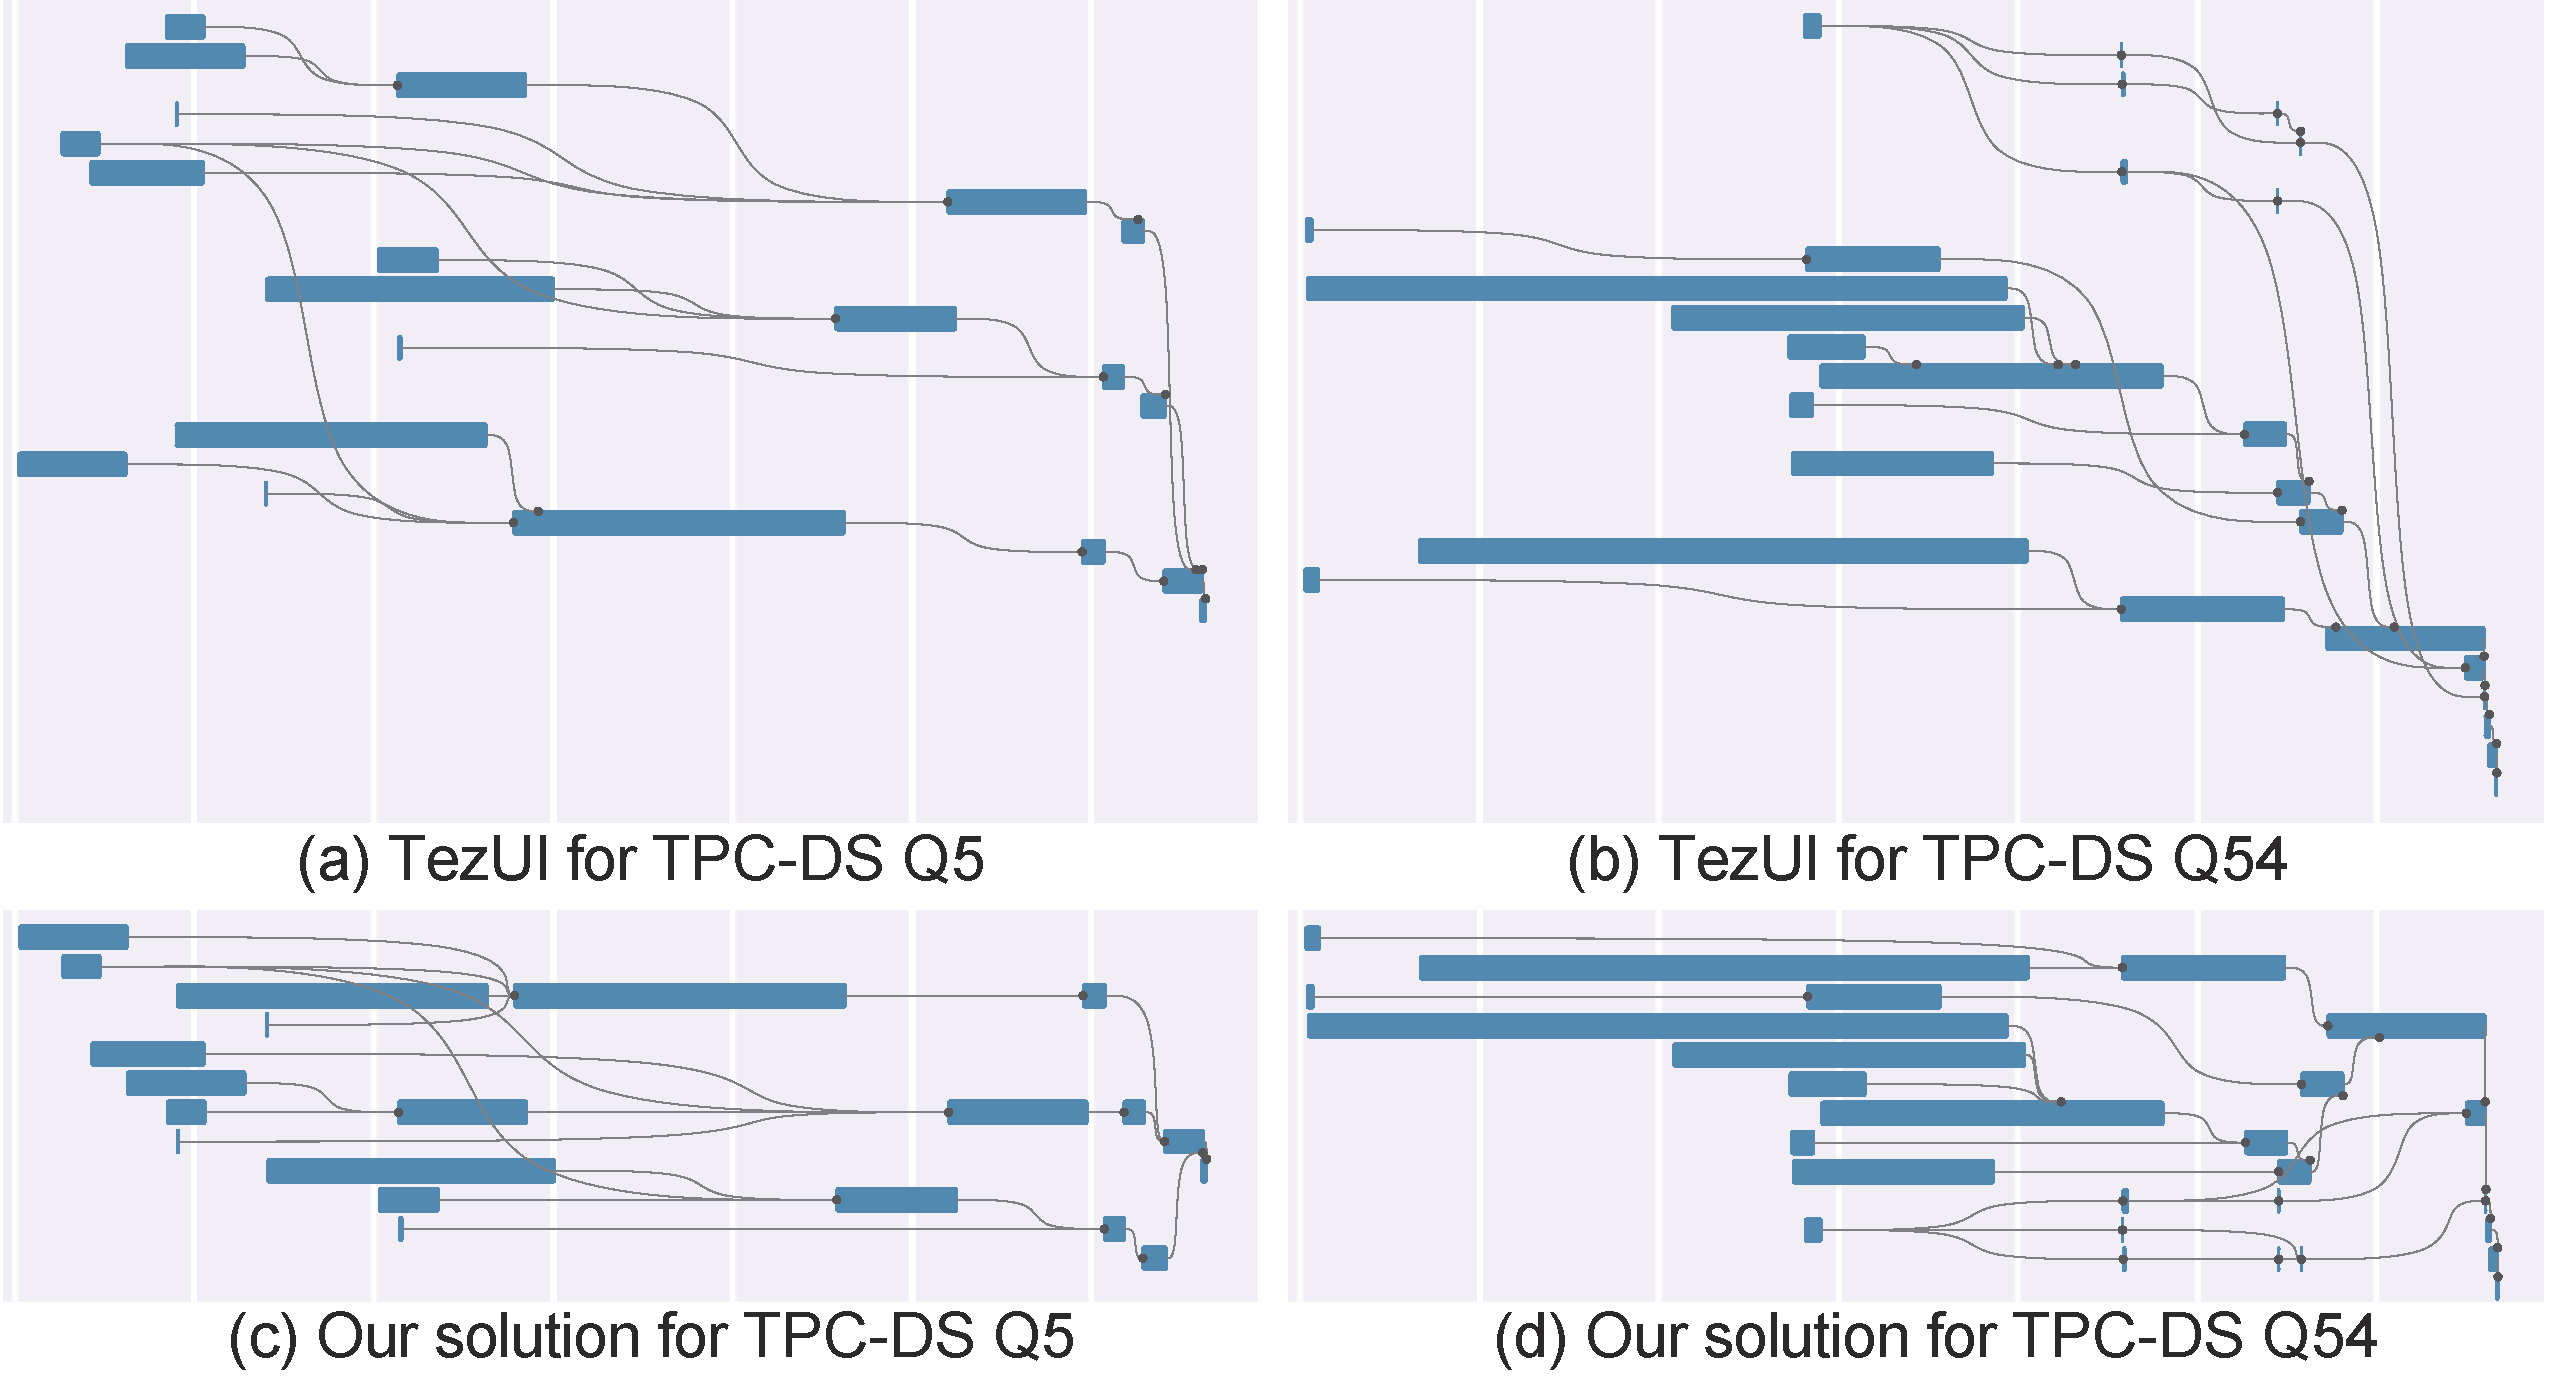
\includegraphics[width=0.44\textwidth]{figures/visualization/exeprogressSDS.pdf}
	\vspace{-3mm}
	\caption{Comparing TDAG layout methods}
	\label{fig:layout}
	\vspace{-3mm}
\end{figure}

\begin{figure}
	\centering
	\small	
	\includegraphics[width=0.42\textwidth]{figures/visualization/TDAG-new-algo.pdf}
	\vspace{-3mm}
	\caption{Workflow of our TDAG layout algorithm}
	\label{fig:layoutmethod}
	\vspace{-5mm}
\end{figure}




To effectively visualize the progress of job execution, it is essential to display the timing information, including start time, end time, and time usage, as well as the dependencies among jobs in the query logical plan (\textbf{T1.1.1} and \textbf{T1.1.3}). This data can be modeled as a DAG enhanced with temporal information (TDAG).
Existing tools (e.g., TezUI and SparkUI) enhance traditional Gantt chart with links to visualize the TDAG. 
This solution is limited because (i) it does not consider the visual clutter caused by the many job dependencies in the execution plan; and (ii) it does not scale to large TDAG as screen space is not utilized efficiently. \autoref{fig:layout} (a) and \autoref{fig:layout}(b) show its visualizations for the TDAG of TPC-DS query 5 and 54, respectively. The edges and nodes are crossed in \autoref{fig:layout}(a) due to complex job dependencies, and there is a large blank space in the left bottom part of \autoref{fig:layout}(b).


To tackle the two challenges, we propose a novel TDAG layout method illustrated in \autoref{fig:layoutmethod}. It includes the following steps:

\squishlist
\item \stitle{Step 1} We first simplify the job DAG, see \autoref{fig:layoutmethod}(a), to a job dependency tree in \autoref{fig:layoutmethod}(b).
In particular, the output of a job can be the input of many jobs (e.g., $\geq 2$ jobs), and we only preserve the edge from a job to its out-neighbor job with the earliest start time.
For example, the output of job $1$ serves as input for jobs $4$ and $6$ but the start time of job $4$ is earlier than job $6$. Thus, we only keep the edge from job $1$ to job $4$ in the simplified job tree in \autoref{fig:layoutmethod}(b).
TDAG simplification is conducted to (i) preserve the starting time order of the jobs, and (ii) keep dependent jobs close to each other to prevent visual clutter.

\item \stitle{Step 2} We then plot a rectangle for each job by using the length of the rectangle to indicate job duration and sort the jobs by their start time, as shown in \autoref{fig:layoutmethod}(c).
This follows human reading habit (i.e., reading from top to bottom) and plots the job starting earlier in a higher position. 

\item \stitle{Step 3} We next adjust the layout of jobs by utilizing the job dependencies in the simplified tree. In particular, we check the jobs the top to bottom. For each job, if its out-neighbor job could be placed in the same row with it (i.e., non-overlapping), we move the out-neighbor to the same row with it, and add an edge between these two jobs. 
For instance, the time duration of job $1$ does not overlap with the time duration of its out-neighbor job $4$, thus we plot jobs $1$ and $4$ in the first row, see \autoref{fig:layoutmethod}(c).

\item \stitle{Step 4}  Last, we refine TDAG layout by (i) adding the other edges in the job DAG, for example, jobs $1$ and $6$ in \autoref{fig:layoutmethod}(e), and (ii) reducing the space by combining the rows that do not overlap, for example, job $3$ and job $5$ are plotted in the same row in \autoref{fig:layoutmethod}(e).
\squishend




%We visualize the TDAG of TPC-DS query 5 and query 54 by our TDAG layout algorithm in \autoref{fig:layout}(c) and (d), respectively. Compared with the visualizations produced by Tez UI \autoref{fig:layout}(a) and (b), our visualizations are obviously better. In particular, visual clutter is significantly reduced in our visualization because we consider the dependencies among the jobs via the simplified tree. Moreover, our visualizations take much smaller screen space because our adjustment considers job dependencies and time duration.    
We visualize the TDAG of TPC-DS query 5 and query 54 by our TDAG layout algorithm in \autoref{fig:layout}(c) and \autoref{fig:layout}(d), respectively. 
\qm{
%	Compared with the visualizations produced by Tez UI \autoref{fig:layout}(a) and (b), our visualizations reduce the visual clutter because we consider the dependencies among the jobs via the simplified tree. Moreover, our visualizations take smaller screen space because our adjustment considers job dependencies and time duration.    
%	Compared with the visualizations produced by Tez UI \autoref{fig:layout}(a) and (b), the visualization generated by our approach have two benefits:1) since our approach considers the topological structure of execution plan, the visualization has less visual clutter because it has few crossing among the links and rectangles; 2) the proposed visualization task smaller screen space because the algorithms considers both job dependencies and time duration. 
	When compared with the visualizations produced by Tez UI \autoref{fig:layout}(a) and \autoref{fig:layout}(b), 
	the visualization generated by our approach offers two advantages: (1) our visualization takes into account the topological structure of the execution plan, resulting in reduced visual clutter as there are fewer crossings among the links and rectangles; (2) our proposed visualization optimizes screen space utilization by considering both dependencies and time duration, allowing for a more efficient visualization.
}


We enhance the \vtitle{job view} with two visual designs (i.e., parallelism and phase mode) to show more information for each job (\textbf{T1.1.2}). 

\sstitle{Parallelism mode} we embed the task parallelism (i.e., number of running tasks) into the job rectangle. Specifically, we use a 1D-heatmap to visualize the number of active tasks over time, as shown in \autoref{fig:teaser}(b). 
A gradient color from white to dark blue encodes the number from one to the maximum number of active tasks for the job. We color the number zero with a special color (e.g., gray) as zero indicates that the execution of the job is suspended and users should pay attention. 

\sstitle{Phase mode} we visualize the percentage of time used by the three phases of each job, as shown in \autoref{fig:teaser}(b1), and use three colors to indicate the three phases.  
This allows users to better understand the jobs, e.g., classifying them into I/O-bounded or compute-bounded jobs.



\subsubsection{Performance matrix}\label{sec:taskmachinepair}
As shown in \autoref{fig:teaser}(c), performance matrix is designed to show the anomaly degree of jobs and machines such that users can narrow down the scope of exploration (\textbf{T2}). 
Existing tools~\cite{elephant, prometheus} propose different scoring schemes for different anomaly types, e.g., data skew and memory overload. This approach is limited as it is difficult to encompass all possible anomalies. We adopt a different approach, which considers the execution statistics of the tasks and quantifies how far they deviate from ideal distributed parallel execution. 
We believe a component is \qm{worth paying attention to} if it deviates far from ideal, and we leave it to the users to determine the specific anomalies by inspecting the views we provided.
In the ideal case, all tasks of a job have a similar workload and run in parallel, which results in similar time usage and high parallelism for these tasks.
On this basis, we propose two novel anomaly scores to analyze the tasks of a job, i.e., \textit{abnormal parallelism score} ($\aps$) and \textit{abnormal duration score} ($\ads{}$).

\begin{figure}
	\centering
	\small
	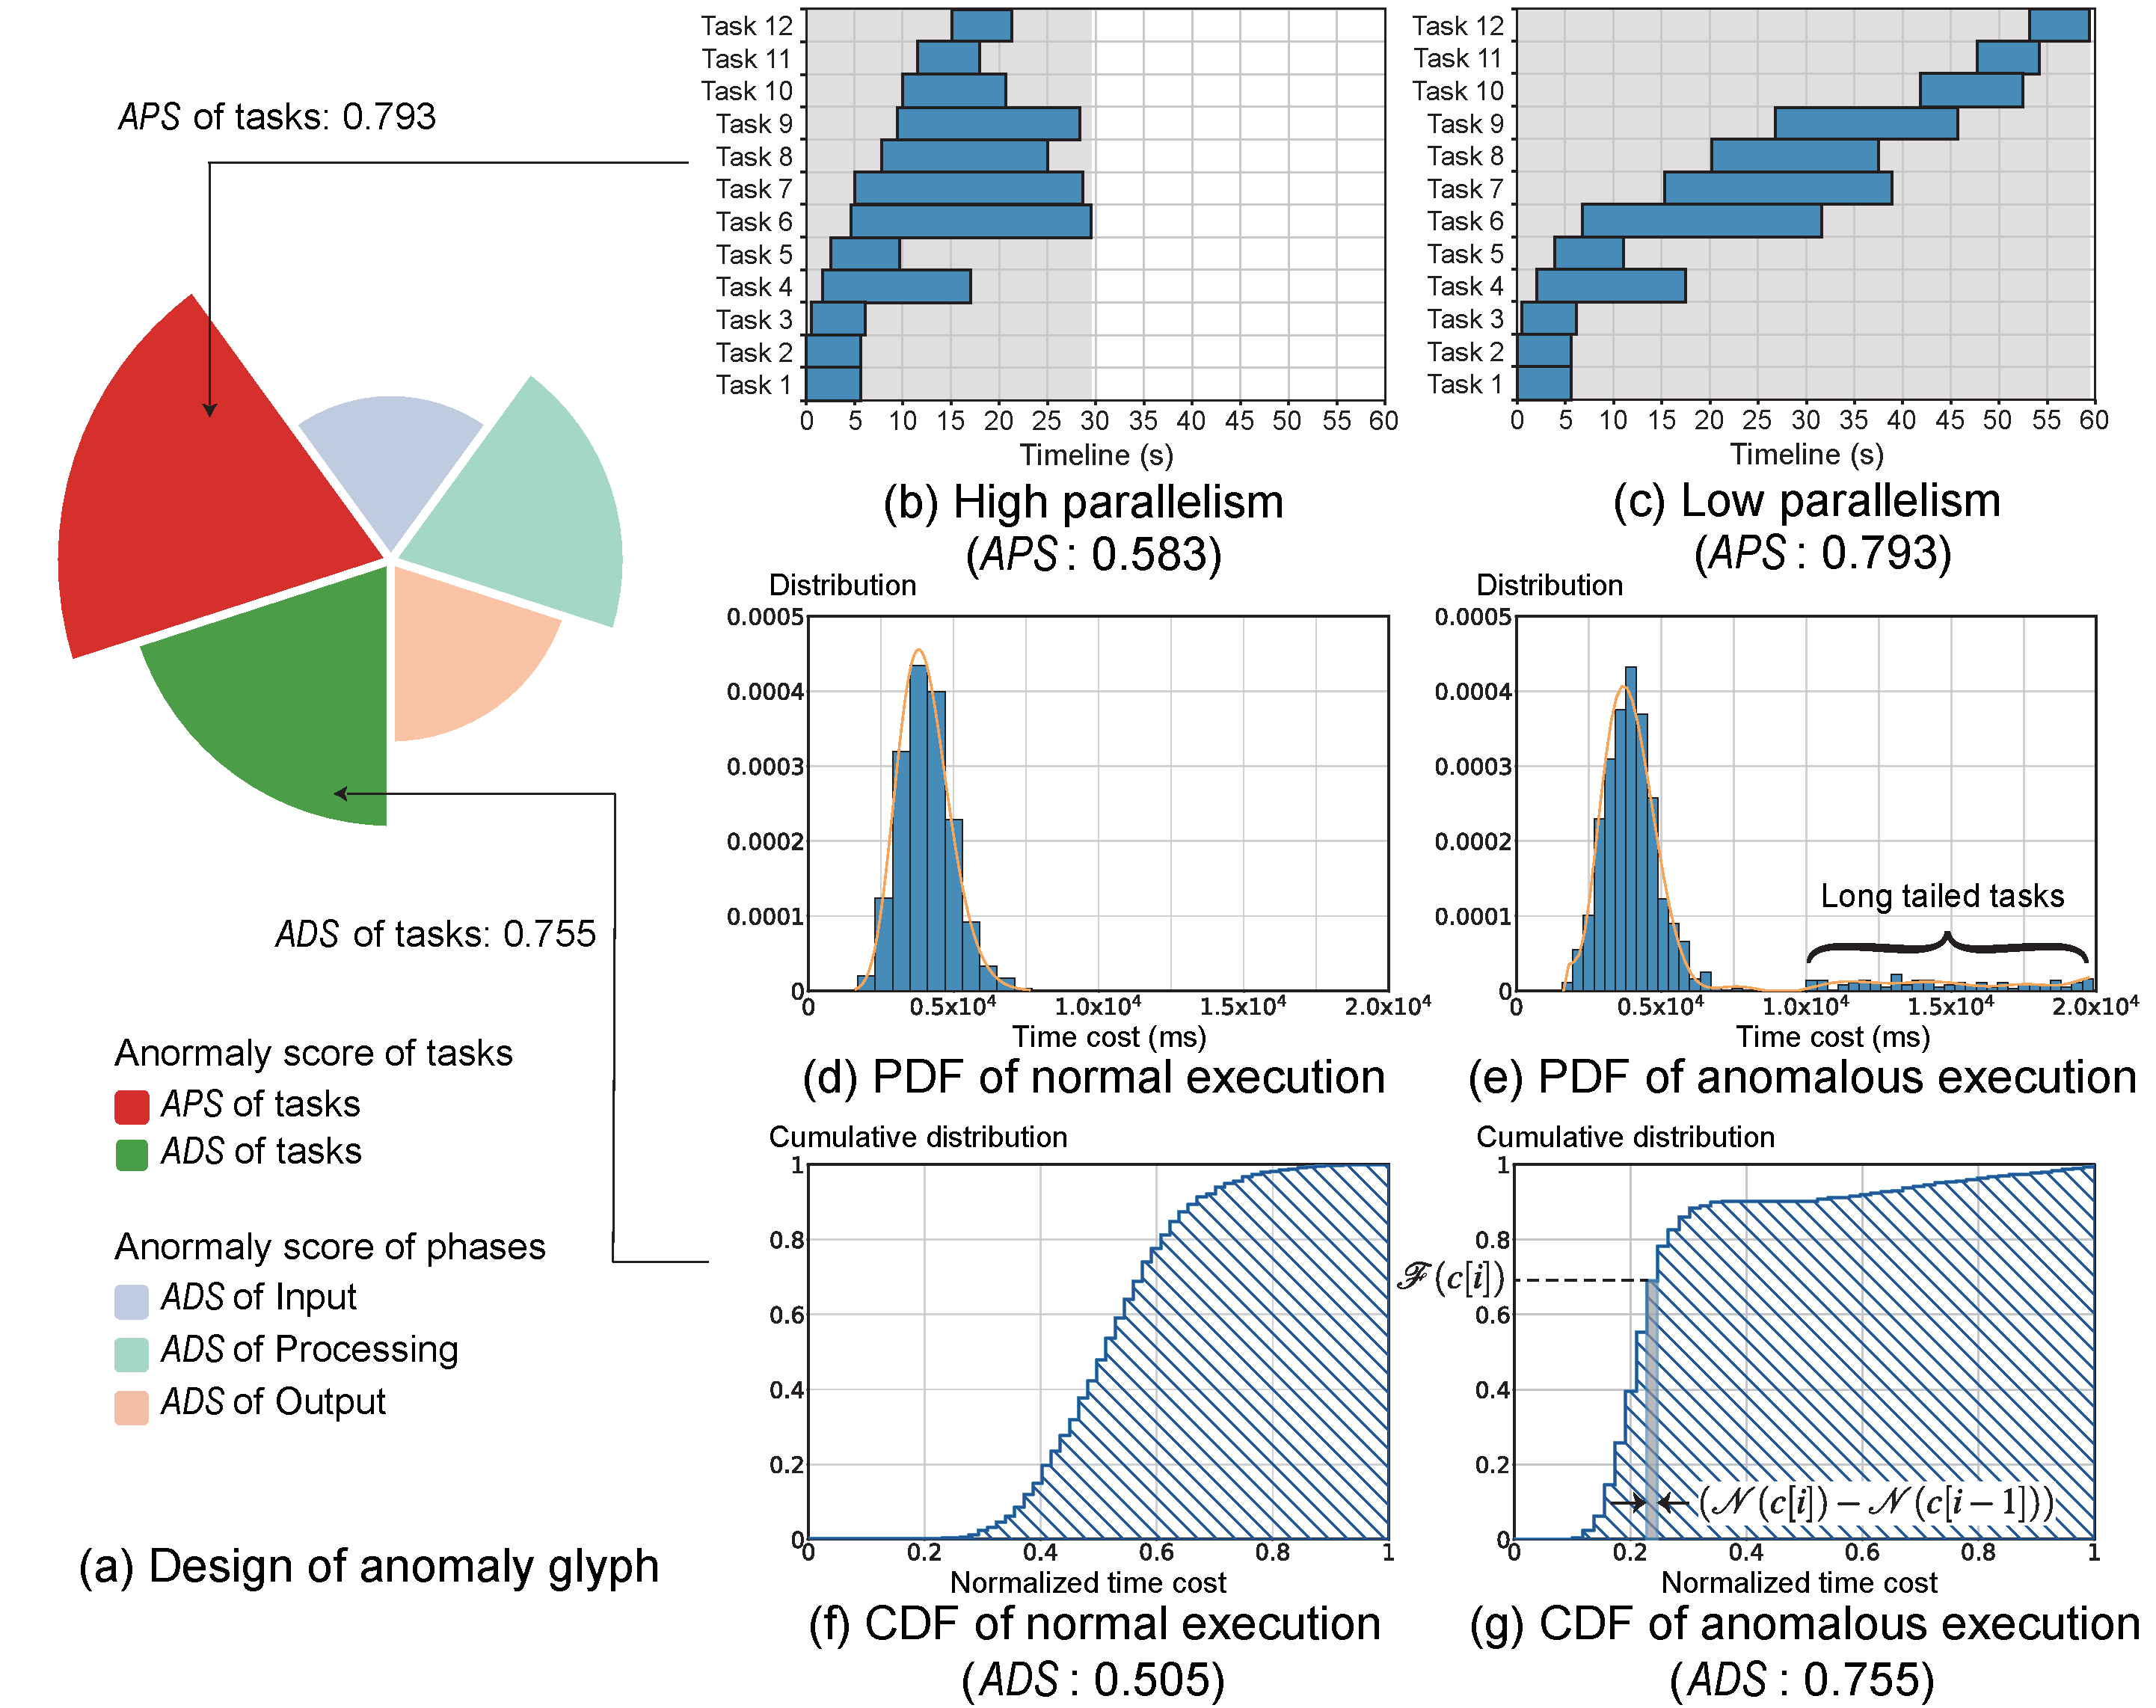
\includegraphics[width=0.42\textwidth]{figures/dataprocess/anomaly_illustration_vis2023.pdf}
	\vspace{-3mm}
	\caption{Illustration of anomaly scores}
	\label{fig:score}
	\vspace{-5mm}
\end{figure}

\stitle{Abnormal parallelism score ($\aps$)} $\aps$ measures how well the tasks of a job are parallelized, \qm{how many jobs share the similar start time and end time.}
%\qm{Parallelism refers to the synchronization of task start and end times.}

For example, the tasks in \autoref{fig:score}(b) are paralleled better than the tasks in \autoref{fig:score}(c) as the tasks are better overlapped in time and more of them run concurrently. Denote the task set of job $j$ as $T_j = \{t_j[1], \cdots, t_j[n]\}$, the $\aps$ of $T_j$ is defined as:
$$\aps(T_j) = 1 - \frac{\sum_{i^=1}^{n} (t_j[i]_e - t_j[i]_s)}{n \times (j_e - j_s)}.$$
Intuitively, the second term of $\aps$ measures the ratio between the area of all tasks (the bars in \autoref{fig:score}(b) and \autoref{fig:score}(c)) over the area of the job rectangle (the gray area in \autoref{fig:score}(b) and \autoref{fig:score}(c)). If all tasks have the same time usage and run concurrently, $\aps$ will be 0, and thus large $\aps$ indicates anomalous. For instance, the $\aps$ for the tasks in \autoref{fig:score}(b) and \autoref{fig:score}(c) are 0.583 and 0.793, respectively, indicating that \autoref{fig:score}(c) deviates further from the ideal.    



\stitle{Abnormal duration score ($\ads$)}
It is observed that the time usage of the tasks in a job is
 usually tightly clustered and unexpectedly long query execution time is usually caused by a few long-running tasks~\cite{tan2010visual}, which causes a long tail in the time usage distribution.
For instance, \autoref{fig:score}(d) and \autoref{fig:score}(e) illustrate the task time usage distribution of two jobs, and the distribution in \autoref{fig:score}(e) has a long tail, which results in a long job time usage.

We use $\ads$ to measure the significance of long tail tasks.
Denote the task set of job $j$ as $T_j = \{t_j[1], \cdots, t_j[n]\}$ and the time usage of the tasks as $C_j = \{c[1], c[2], \cdots, c[m] \}$ when sorted in ascending order. The $\ads$ of $T_j$ is defined as follows:
$$
\ads(T_j) =\sum_{i=2}^{m}  F(c[i]) \cdot (N(c[i]) - N(c[i-1]))
$$
where $F(c[i])$ is the cumulative distribution function of task time usage, which returns the percentage taken by the tasks with shorter time usage than $c[i]$ in all tasks, and
$N(c[i]) = \frac{c[i]-c[1]}{c[m]-c[1]}$ is the normalized value of $c[i]$ and is in the range of 0 to 1 for all tasks. Intuitively, $\ads$ measures the area covered under the cumulative distribution of task time usage, the gray areas in Figures~\ref{fig:score}(f) and (g), and long tail tasks will enlarge the area and $\ads$.  
The intuition of the $\ads$ score is measuring the cumulative distribution of all tasks. 
The $\ads$ score will be large if some tasks have unexpectedly long running time. For instance, the $\ads$ of the tasks in Figures~\ref{fig:score}(d) and (e) are 0.505 and 0.755, respectively, indicating that \autoref{fig:score}(e) has a more severe long tail problem.     


We scale the $\aps$ and $\ads$ scores of a job $j$ by the time usage of the job in the entire query, i.e., $\rho(j) = \frac{j_e - j_s}{C}$, where $C$ is the overall execution time of the query. This allows users to focus on important jobs because even if a short-running job has execution anomalies, its influence on the entire query may still be small. 
Our two anomaly degree scores are generic and can assist analysis at different levels, e.g., job level, task level or phase level. As will be shown later, we also use them to measure the anomaly degree of the three phases in the tasks.


\stitle{Visualization designs for performance matrix} As shown in \autoref{fig:teaser}(c), we use a matrix-based visualization to show the anomaly scores. 
The x-axis and y-axis correspond to the jobs and machines, respectively. 
The first row displays the overall anomaly scores of each job. 
The cell in $m$-th row and $j$-th column displays the anomaly score of job $j$'s tasks that are executed on machine $m$. 
\qm{We sort the columns and rows by descending order of their average anomaly score. 
In cases where the number of machines or jobs is particularly large, we preserve only the top k jobs (default value: 30) and top n machines (default value: 10) as specified by the analyst. 
}
As illustrated in \autoref{fig:score}(a), we show the anomaly scores by Nightingale's chart~\cite{brasseur2005florence}, which is commonly used to visualize multi-attribute data~\cite{zhao2017skylens}. 
The radius of each sector represents the value of an anomaly score while the color represents the granularity (e.g., task- or phase- level) of anomaly and can be configured by users. 
The color encoding for the phases is coincident with the job progress in \autoref{fig:teaser}(b1).
%The jobs are ordered 	from left to right based on the sum of their anomaly values.



\subsubsection{Task view}\label{sec:task}
The \vtitle{task view} allows users to analyze the tasks in detail (\textbf{T1.1.3}) and consists of multiple panels . The panel at the top of \vtitle{task view} shows all tasks of the  query, and the remaining panels display the tasks executed on each machine.
Each panel displays the machine id (e.g., dbg19) at the top and uses a scatter plot-based visualization to plot the tasks as points in a square view, as shown in \autoref{fig:distribution}(a).

The visualization provides two kinds of task information using different parts: (i) \textit{Temporal distribution}, which depicts the start time, end time and time usage of the tasks, see the top-right triangle in \autoref{fig:distribution}(a); and (ii) \textit{Data dependency distribution}, which embeds the data dependencies among the tasks of different jobs, as shown by the bottom-left triangle in \autoref{fig:distribution}(a).



\begin{figure}
	\centering
	\small
	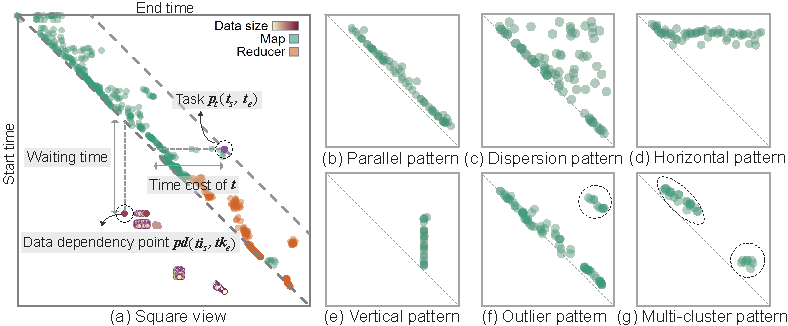
\includegraphics[width=0.48\textwidth]{figures/visualization/distributionview_revision.pdf}
	\vspace{-2mm}
	\caption{\vtitle{Task view} and task time usage patterns}
	\label{fig:distribution}
	\vspace{-6mm}
\end{figure}

\stitle{Temporal distribution}
Existing tools (e.g., SparkUI~\cite{sparkui} and Inviso~\cite{inviso}) usually employ Gantt chart to visualize the tasks, which are limited for two reasons: (i) Gantt chart causes severe visual clutter when visualizing massive (e.g., thousands) tasks; (ii) it is difficult to compare the time usage of different tasks as Gantt chart lacks proper alignment. 

To tackle these limitations, we plot the tasks as points in a square view.
In particular, we use the x-axis of the square view to represent the task start time and the y-axis to represent the task end time, which makes task $t$ a point, i.e., $p_t(t_s, t_e)$, in the square view. 
\qm{This configuration of the axes aligns with the conventional reading patterns observed in humans when browsing websites.} 
We use green and orange colors to encode the tasks of map and reducer job, respectively.
As shown in \autoref{fig:distribution}(a), this scatter point view design has several properties:
first, all points are in the top-right half of the square view because $t_e > t_s$ holds for all tasks;
second, the horizontal distance between the diagonal line and point $p_t$ encodes the time usage of task $t$, as illustrated by the dashed line in \autoref{fig:distribution}(a).
For interactive analysis, when a user moves the mouse on a task $t$, we plot a gray dashed auxiliary line that is parallel to the diagonal line and passes through point $p_t$ to show the time usage of the task. \qm{More importantly, for all tasks of a job, the distribution patterns of the points in the scatter point view reveal the query execution status and provide useful hints for the root causes of execution problems.
Figures~\ref{fig:distribution}(b) to (g) show the most representative patterns we observed in the production environment. We provide our observed hints of them below. 
}

\squishlist
\item \sstitle{\textbf{Parallel} pattern in \autoref{fig:distribution}(b)} it suggests that all tasks have similar time usage, resulting in points that are parallel and close to the diagonal line. \qm{A dense and parallel pattern indicates the query is executed smoothly.}
\item \sstitle{\textbf{Dispersion} pattern in \autoref{fig:distribution}(c)} it means that the tasks of a job have different start time and end time.\qm{
It suggests that these tasks may encounter multiple problems at the same time, such as insufficient resources, load imbalances, and limited executors, etc.
}

\item \sstitle{\textbf{Horizontal} pattern in \autoref{fig:distribution}(d)} it means all tasks start at almost the same time but end at different times.\qm{
As a special case of Dispersion pattern, it indicates the number of containers is enough, since all tasks can be executed at the same time.
}
\item \sstitle{\textbf{Vertical} pattern in \autoref{fig:distribution}(e)} it shows that the tasks finish together.\qm{
The vertical pattern appears typically because these tasks are all waiting for input data from a same upstream task which is usually the bottleneck.
}
\item \sstitle{\textbf{Outlier} pattern in \autoref{fig:distribution}(f)} it reveals that several tasks have much longer time usage than others. \qm{It indicates that these tasks may suffer from data skewness or deadlock. These tasks are largely the bottleneck of the query execution.
}
\item \sstitle{\textbf{Multi-cluster} pattern in \autoref{fig:distribution}(g)} it shows several separated groups of tasks. \qm{It usually indicates the execution of the job is interrupted for a period of time, which is usually caused by hardware problems or inefficient resources.}
\squishend



\stitle{Alternative design}
Several design alternatives for \textit{distribution view} are considered, including the Gantt chart, Marey's chart and Arc chart, which have been used in related research work and software. 
\autoref{fig:alt} shows the implementation of these designs and our methods with the same dataset. The green and orange colors indicate Map and Reducer tasks, respectively. 
Gantt chart is the most intuitive design to visualize the tasks through rectangular bars, however, when data is large, the height of bars will become too narrow to be observed. The other two designs all use lines (curves) instead of bars to show the temporal information of tasks. Marey's chart uses two horizontal axes to indicate the start time and end time, thus the task can be represented as a line connecting the two axis. Arc chart uses arcs to show the tasks, with two end points of the arc indicating the start time and end time. 
All these designs work well when the data size is small. However, in our application, the number of tasks will reach tens of thousands, which results in different problems for each design. For instance, the height of bars becomes too narrow to observe in  Gantt chart; Marey's chart and Arc chart all have serious visual clutter results from the overlap and cross of lines (curves), especially for Marey's graph, the orange lines are too dense to reflect any patterns. 

\begin{figure}[t]
	\centering
	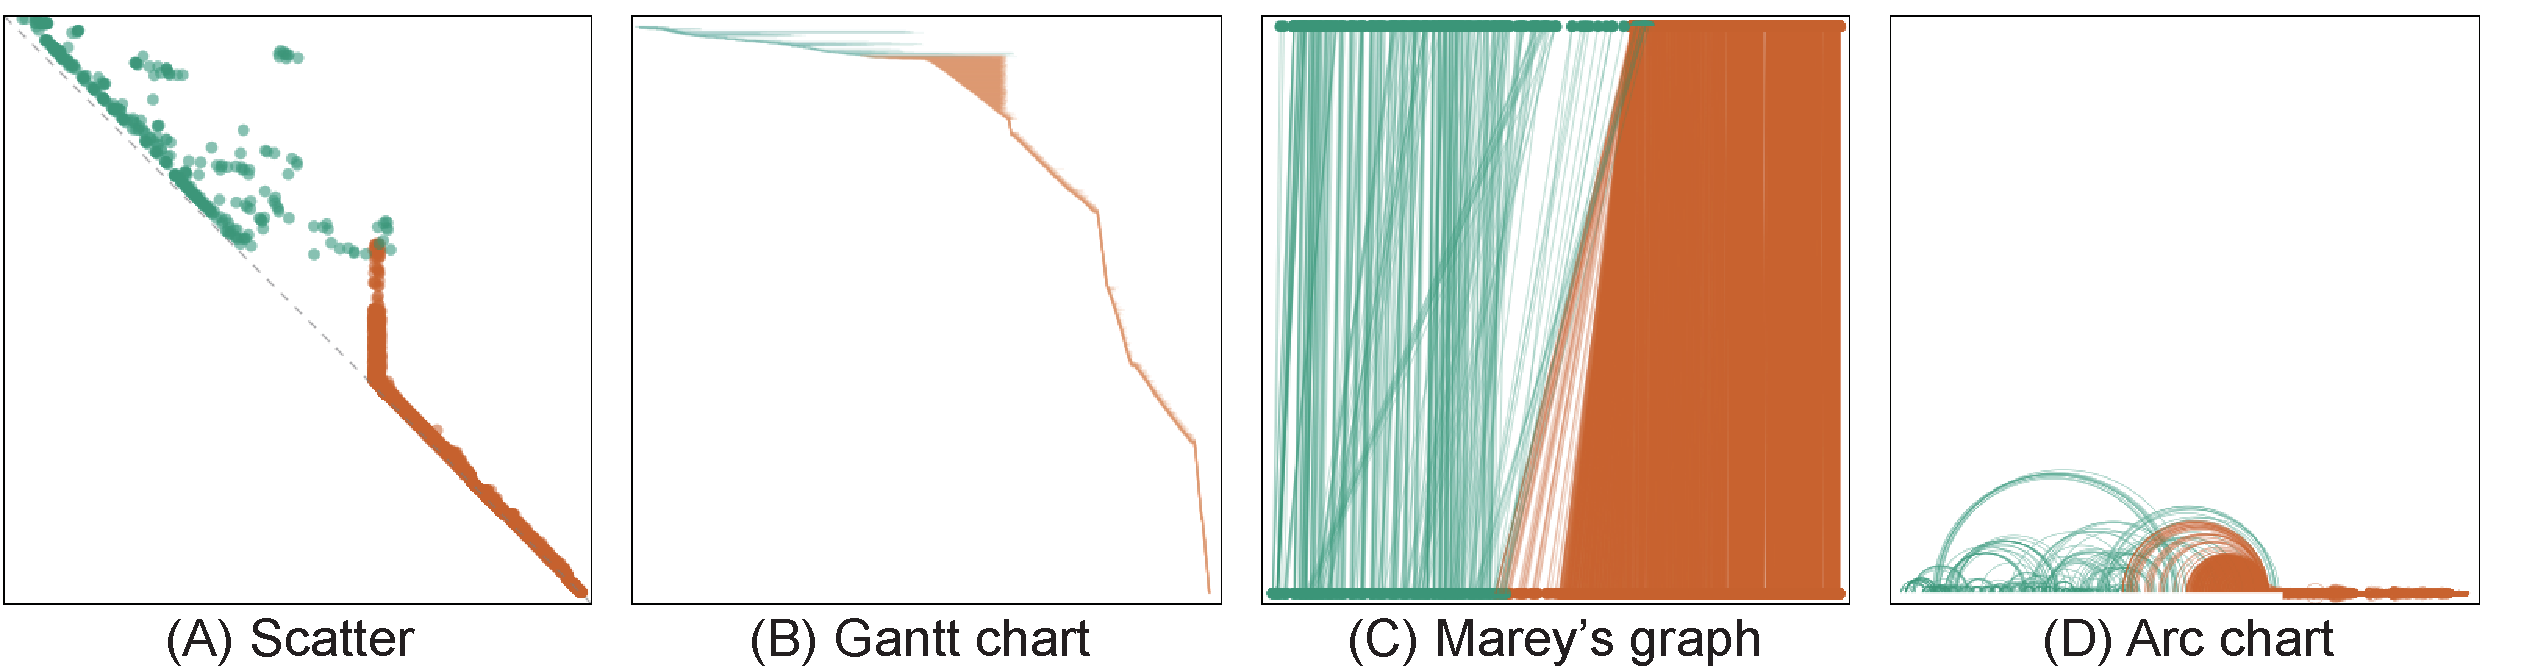
\includegraphics[width=0.48\textwidth]{figures/visualization/alternative_design.pdf}
	\vspace{-3mm}
	\caption{Alternative design of task/dependency distribution}
	\label{fig:alt}
	\vspace{-8mm}
\end{figure}


\stitle{Data dependency distribution}
Consider two tasks $ti$ and $tk$ with data dependency, and the output of $ti$ is used as input by $tk$.
The start time of $tk$ should be later than the end time of $ti$ in the idle case but the opposite may happen in abnormal cases (usually caused by the resource scheduler).
To visualize these abnormal cases, 
we show the data dependency of $ti$ and $tk$ by plotting point $p_d(tk_s, ti_e)$ in the square view. 
As $tk_s<ti_e$, all these abnormal tasks are in the bottom-left half of the square view, as shown by the purple points in \autoref{fig:distribution}(a). Thus, the dependency distribution does not interfere with the temporal distribution, which is in the top-right half.     
We provide several interaction mechanisms in task distribution. For example, once a task is selected, its dependencies, upstream tasks and downstream tasks will be highlighted in red and blue colors, respectively. 
%Interactions such as semantic zoom and drag are supported to locate the details of interests.  

\subsubsection{Auxiliary views and interaction designs}\label{sec:other}
We provide a suite of auxiliary views and rich cross-view interactions in \qevis{} to help users explore query execution progress. Due to space limitation, we only present two auxiliary views (i.e., \vtitle{entity list} and \vtitle{profiling view}) and refer the interested readers to our GitHub repository for the other views (e.g., \vtitle{query list} in \autoref{fig:teaser}(a)).

\sstitle{Entity list} it shows detailed statistics of each job row by row, shown in \autoref{fig:teaser}(e). 
Users can click on the triangle at the leftmost side of each job (i.e., job level) to enter the machine level. 
By clicking the triangle at the machine level, all tasks executed by the machine will be listed. 
To visualize the features of tasks, we implement two visualization forms, i.e., rug plot~\cite{rug_plot} and Gantt chart, that will be selected automatically based on the features of interest.
Besides time usage, \vtitle{entity list} also allows users to select other features of interest (e.g., read/write data size) through the dropdown at the top of this view.


\sstitle{Profiling view} it is embedded into each panel in the \vtitle{task view} and consists of a suite of visualizations to show execution statistics such as task parallelism and system hardware usages as illustrated in \autoref{fig:teaser}(f).
For single variate features such as task parallelism and memory usage, we use the line chart, which can show the temporal change of the value. 
For multiple variate features such as CPU usage and Disk IO, we use a heatmap, which is widely used to visualize multiple values.


\stitle{The design of interactions}
\qevis{} supports flexible interactions and cross-view linkage to facilitate multi-view exploration. 
For example, when the user hovers the mouse on a job in the \vtitle{job view}, shown as the purple boundary in \autoref{fig:teaser}(b), all tasks of this job will be highlighted in the \vtitle{task view}, as purple points in \autoref{fig:teaser}(d). 
Conversely, if the user hovers the mouse on a task point in the \vtitle{task view}, the corresponding job in the \vtitle{job view} and \vtitle{entity list} will be highlighted. 
Moreover, when the user clicks on points in the \vtitle{task view}, the \vtitle{entity list} will be expanded to show the corresponding tasks and execution machines, shown as the purple items in \autoref{fig:teaser}(e). 
When the user puts the mouse on an element for more than three seconds, a widget showing detailed information about the element will be displayed. 
Shown as \autoref{fig:teaser}(d2), when we put the mouse on the purple task, the task information such as data read, records processed, and time costs of each phase are displayed. 








\section{Empirical Evaluation}\label{sec:eval}

%In this section, we evaluate the effectiveness of \qevis{} three case studies and user interviews. 
%Specifically, we show how \qevis{} helps domain users understand query execution and pinpoint problems with three real cases from the production environment. 
%Then we invite engineers from our industry partner to use our system and collect their feedback.
In this section, we show how \qevis{} helps domain users understand query execution and pinpoint problems with three real cases from the production environment. 
Subsequently, we invite engineers from our industry partner to use our system and collect their feedback.

\subsection{Case study} \label{sec:case}

%$\qevis{}$ has been deployed in the production environment of Huawei Cloud and is widely used by software engineers.
$\qevis{}$ has been deployed in the production environment and is widely used by software engineers.
Usually, our users are interested in queries that run longer than expected because they degrade system throughput. 
In this section, we demonstrate the effectiveness of \qevis{} via three use cases \qm{about slow query} in production, which identifies hardware, system and data problems during query execution, respectively.


\subsubsection{Identifying hardware problem} \label{sec:systemproblem}
\autoref{fig:teaser} shows how \qevis{} visualizes a long running query (i.e., 623 seconds) from a business intelligence application and we analyze it as follows.

\stitle{Step 1: investigate the performance bottleneck via \textit{job view}}
The \textit{job view} of the query is shown in \autoref{fig:teaser}(b).
Visually, job M1 has a very long running time.
More importantly, there is a large gray region in job M1, which means that the number of running tasks is 0 in this region according to the design of job rectangle in \autoref{sec:job}.
Thus, job M1 is the cause of long execution.


\stitle{Step 2: inspect job M1's task execution pattern via \textit{task view}}
To find the reasons that cause the gray region for job M1 in the \textit{job view}, we analyze the tasks of job M1 via the \textit{task view}.
When hovering the mouse on the job rectangle of M1, its associated tasks are highlighted with purple color in the \textit{task view}, see \autoref{fig:teaser}(d). 
We observe that the tasks of job M1 form two groups (i.e., \textbf{multi-cluster} pattern) that are far away from each other, as illustrated by the two dashed ellipses in \autoref{fig:teaser}(d). 
As discussed in \autoref{sec:task}, the multi-cluster pattern suggests that the tasks of job M1 are not executed properly due to machine problems.

\stitle{Step 3: locate the problematic machine via \textit{entity list}}
We know that the long running query is caused by machine problems but it is difficult to pinpoint the problematic machines as the production cluster is large.
Fortunately, \qevis{} provides the \textit{entity list} to map tasks to their executing machines.
By checking the \textit{entity list}, as illustrated by the rows with purple stroke in \autoref{fig:teaser}(e1), 
we observe that the tasks of job M1 in the right-bottom corner are executed on machine dbg18
%~\footnote{We anonymize the machine identifiers as required by our industry partner.}.
Then, we take a closer look at the tasks executed on dbg18, see \autoref{fig:teaser}(d1).
Compared with the other machines (e.g., dbg16, dbg19, dbg20), the number of tasks executed by dbg18 is quite small,
which suggests that the resource scheduler YARN allocates a small number of tasks to dbg18. 
This confirms that dbg18 is the problematic machine and YARN is aware of this fact during the query execution progress.
%With the conclusion above, we contact the infrastructure team and they confirm with us that the hard disk of dbg18 incurs errors.

Similar analyzing steps are also applied to job M24, which is another long running job in the query. 
We find that the long running time of job M24 is caused by a few straggling tasks on dbg19.
By investigating them, we find that dbg19 has high CPU utilization, see the red regions of the CPU usage heatmap in \autoref{fig:teaser}(f). 
We omit its analyzed steps as they are similar to the steps for job M1. 

To sum up, hardware problems cause the long running query. 
To verify, we remove dbg18 and dbg19, and re-run the query. The running time becomes 200 seconds.
\autoref{fig:teaser}(b1) shows the new \textit{job view}, where the running time of jobs M1 and M24 are much shorter than before.

\qm{
\stitle{Discussion}
%In this case study, the task cross-view linage and task level visualization analysis plays an important role in facilitate the execution exploration. Through the linkage among \vtitle{job view} and \vtitle{task view}, we quickly find the abnormal tasks (the group of late executed tasks) and then find these tasks are executed on a problematic machine which run very few tasks. 
%In this case study, the long execution of query is caused by multiple hardware problem, which is commonly appeared in real applications. The task level visualization of \qevis{} is key to facilitate exploration in this case. It allows users to quickly identify the abnormal tasks. Then we find their commonness through the cross-view linkage (\vtitle{task view} and \vtitle{entity list}), which is that all of these machines are executed on dbg18. Then we use \vtitle{task view} of dbg18 to confirm that the machine is suffering from hardware problem. 
%In this case study, the prolonged query execution is attributed to several hardware issues, a common occurrence in real-world applications. The task-level visualization provided by \qevis{} plays a crucial role in aiding exploration in this particular case. It enables users to promptly identify abnormal tasks. Through cross-view linkage, specifically between the task view and entity list, we determine a common factor: all these tasks are executed on dbg18. Further utilizing the task view of dbg18, we confirm that the machine is indeed experiencing a hardware problem.
%In this case study, the query execution suffers from multiple hardware issues. The \vtitle{task view} of all tasks plays a crucial role in aiding exploration by enabling users to promptly identify the abnormal tasks. The \vtitle{task view} of dbg18 further shows that the machine dbg18 which executes the abnormal tasks is suffering from a hardware problem.
%
%The \vtitle{task view} offered by \qevis{} plays a crucial role in aiding exploration by enabling users to promptly identify the abnormal tasks.  Then we confirm these tasks are executed on the same machine dbg18 through the linkage between \vtitle{task view} and \vtitle{entity list}, and inspect taht this machine is indeed experiencing a hardware problem. 
In this case study, the query execution suffers from multiple hardware issues. The \vtitle{task view} of all tasks plays a crucial role by quickly identifying abnormal tasks. Furthermore, the \vtitle{task view} of dbg18 further shows that the machine dbg18 which executes the abnormal tasks is suffering from a hardware problem. This scenario demonstrates that the visual pattern of tasks is helpful in diagnosing these issues efficiently.
}

\subsubsection{Identifying system problem}
We analyze a query that generates app downloads report for market analysis in this case.
\begin{figure}
	\centering
	\small
	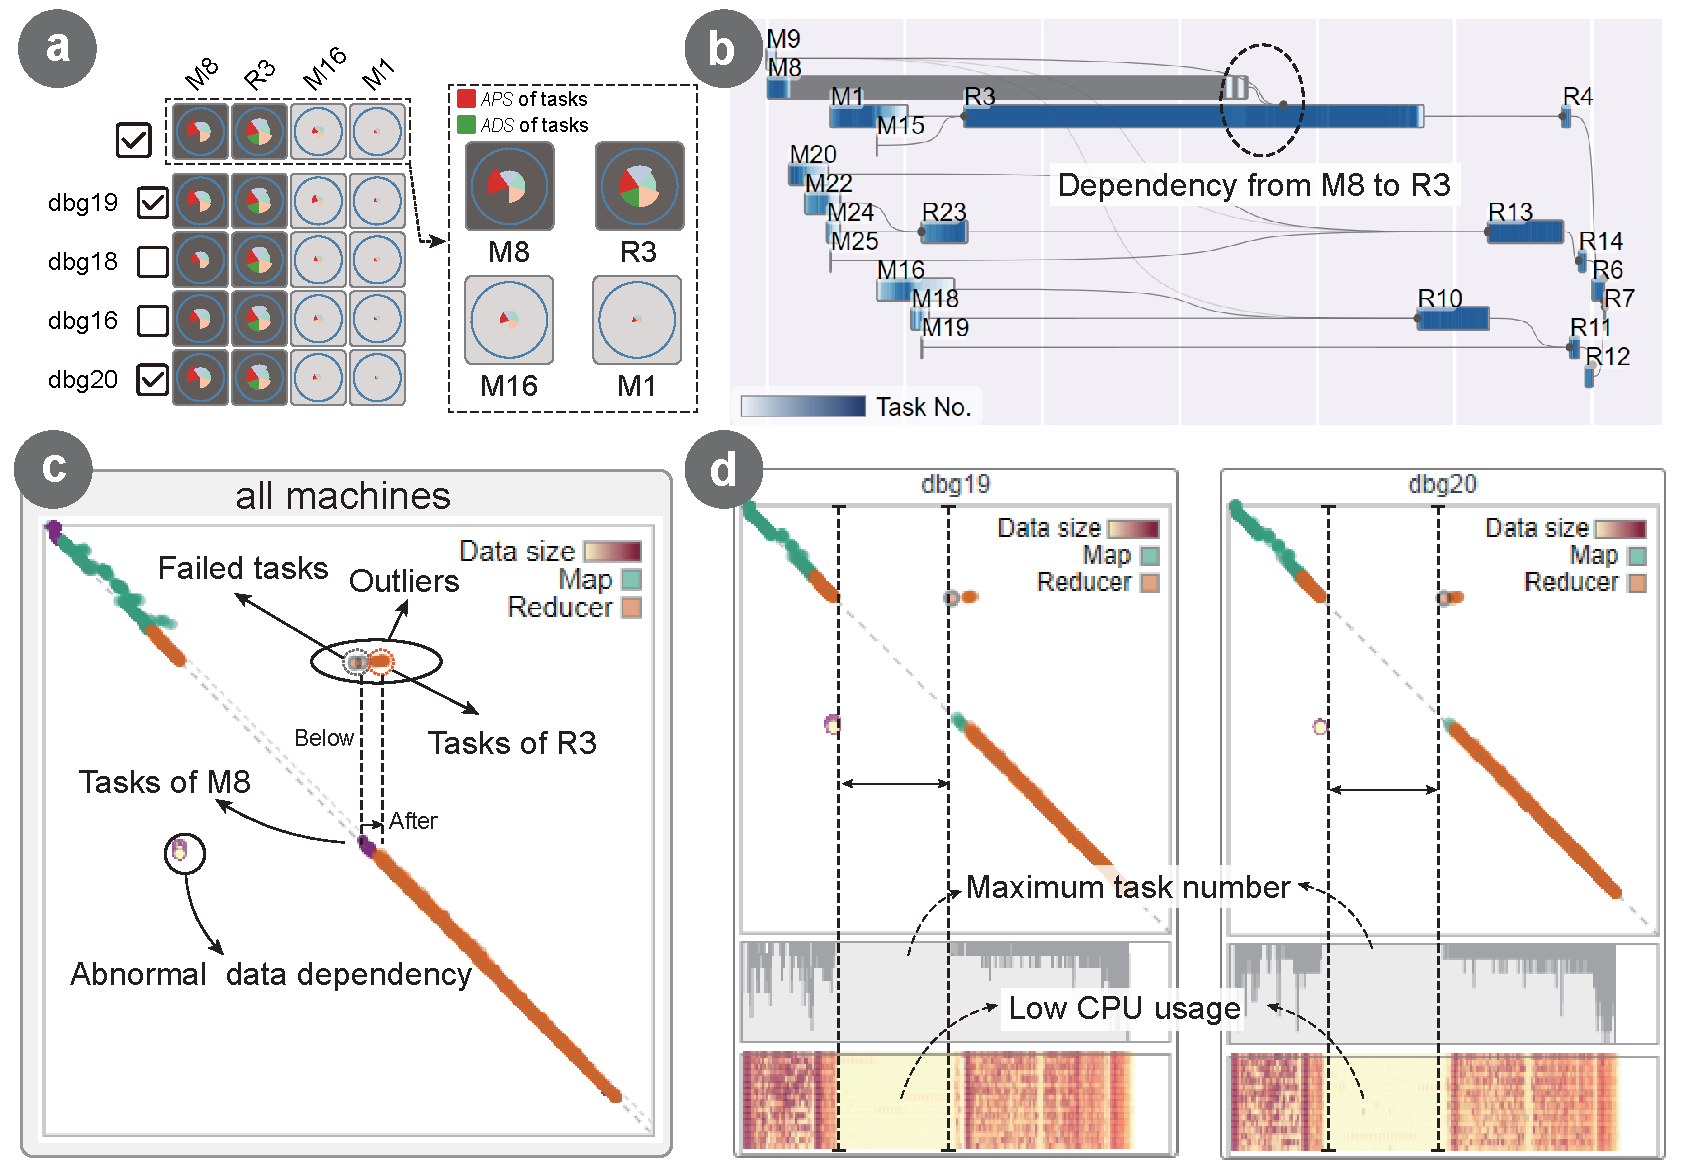
\includegraphics[width=0.46\textwidth]{figures/case_study/CaseStudy2SDS.pdf}  
	\vspace{-3mm}
	\caption{\qevis{} identifies system problem (task deadlock)} 
	\label{fig:casestudy2}
	\vspace{-5mm}
\end{figure}

\stitle{Step 1: observe abnormal jobs via \vtitle{performance matrix}}
As shown by the \textit{performance matrix} in \autoref{fig:casestudy2}(a), the anomaly scores of jobs R3 and M8 are significantly larger than the other jobs, especially the abnormal duration scores (i.e., red sectors). 
Moreover, the green sector (i.e., abnormal parallelism score) of job R3 is also very large.
Since job R3 is the downstream job of M8 as shown in the \textit{job view} in \autoref{fig:casestudy2}(b), 
we conjecture that there is a causal relation between the abnormal behaviors of jobs M8 and R3.


\stitle{Step 2: reveal abnormal data dependency via \vtitle{task view}}
We next perform fine-grained exploration on the tasks via the \vtitle{task view}.
There are several \textbf{outliers}, as highlighted in \autoref{fig:casestudy2}(c).
These outlier tasks can be classified into two categories: (i) failed tasks (the gray points), and (ii) long running tasks (highlighted in orange color).
Interestingly, several tasks of map job M8 are executed immediately after these failed tasks, and then the orange colored tasks of reducer job R3 are executed.
Visually, we can see there are several purple points (i.e., the tasks of job M8) vertically located below the gray points (i.e., failed tasks) and the orange points (i.e., tasks of job R3) are horizontally located after the purple points.
Thus, we confirm that there are abnormal data dependencies among the tasks of jobs M8 and R3, shown as the data dependency points in the left-bottom part of \autoref{fig:casestudy2}(c).


\stitle{Step 3: reason about the failed tasks via \vtitle{profiling view}}
As the \vtitle{profiling view} of the machine is aligned with \vtitle{task view} by time, 
we observe that both dbg19 and dbg20 run the maximum number of tasks during the execution period of these failed tasks, see the range between the two vertical dashed lines for dbg 19 and dbg20 in \autoref{fig:casestudy2}(d). 
However, the CPU utilization of two machines is very low in this period. 
This suggests that the containers of the two machines are fully occupied but no work is done, and thus there is a task deadlock.
In particular, the resource scheduler YARN assigns all containers of dbg19 and dbg20 to the tasks of job R3, and these tasks are waiting for the input data from the upstream tasks of job M8. But the upstream tasks cannot be executed as there are no idle containers, and thus the tasks of jobs M8 and R3 form a circular waiting.
The deadlock is resolved after killing several tasks of job R3, as depicted by the gray colored failed tasks in \autoref{fig:casestudy2}(c).

\qm{
	\stitle{Discussion} 
%	The deadlock appears when the computing resource is limited and too much containers are allocated by source manager(e.g., Yarn). \qevis{} can help analysts identify the deadlock cases with following features: by employing task level visualization with dependencies and properly aligning the timing information of tasks and system profiling.
%Deadlocks occur when computing resources are scarce and an excessive number of containers are allocated by the resource manager (e.g., Yarn). \qevis{} assist analysts to identify deadlock cases through the following features: task-level visualization incorporating dependencies and accurate alignment of timing information from tasks and system profiling. These capabilities enable analysts to gain insights into deadlock situations effectively.
%Deadlocks occur when computing resources are scarce and an excessive number of containers are allocated by the resource manager (e.g., Yarn). \qevis{} assist analysts to identify deadlock cases through the following features: task-level visualization incorporating dependencies and accurate alignment of timing information from tasks and system profiling. These capabilities enable analysts to gain insights into deadlock situations effectively.
%V1
%Deadlocks occur when there's a shortage of computing resources and the resource manager (e.g., Yarn) over-allocates containers. \qevis{} brings following features to address such scenarios: it represents task distribution, enabling users to swiftly identify critical tasks; it displays dependencies that indicate logical relationships among tasks; and it aligns system profiling with execution patterns to illustrate the interplay between resources and execution. The conventional approaches may struggle to manage this situation due to their lack of task oriented visaulization (both task and dependency) and task-system profiling alignment.
%V2
Deadlocks occur when there is a shortage of computing resources and suboptimal task scheduling by resource managers (e.g., Yarn). \qevis{} addresses this by offering following key features: task distribution for quick identification of critical tasks, dependency visualization for understanding logical task relationships and alignment of execution patterns with system profiling to show the interplay between resources and execution. The conventional approaches may struggle to manage this situation due to their lack of task oriented visualization (both task and dependency) and task-system profiling alignment.
}
\subsubsection{Identifying data problem}
We next analyze a query that runs daily for sales analysis, which takes 1200 seconds and is longer than before. 

\begin{figure}[t]
	\centering
	\small
	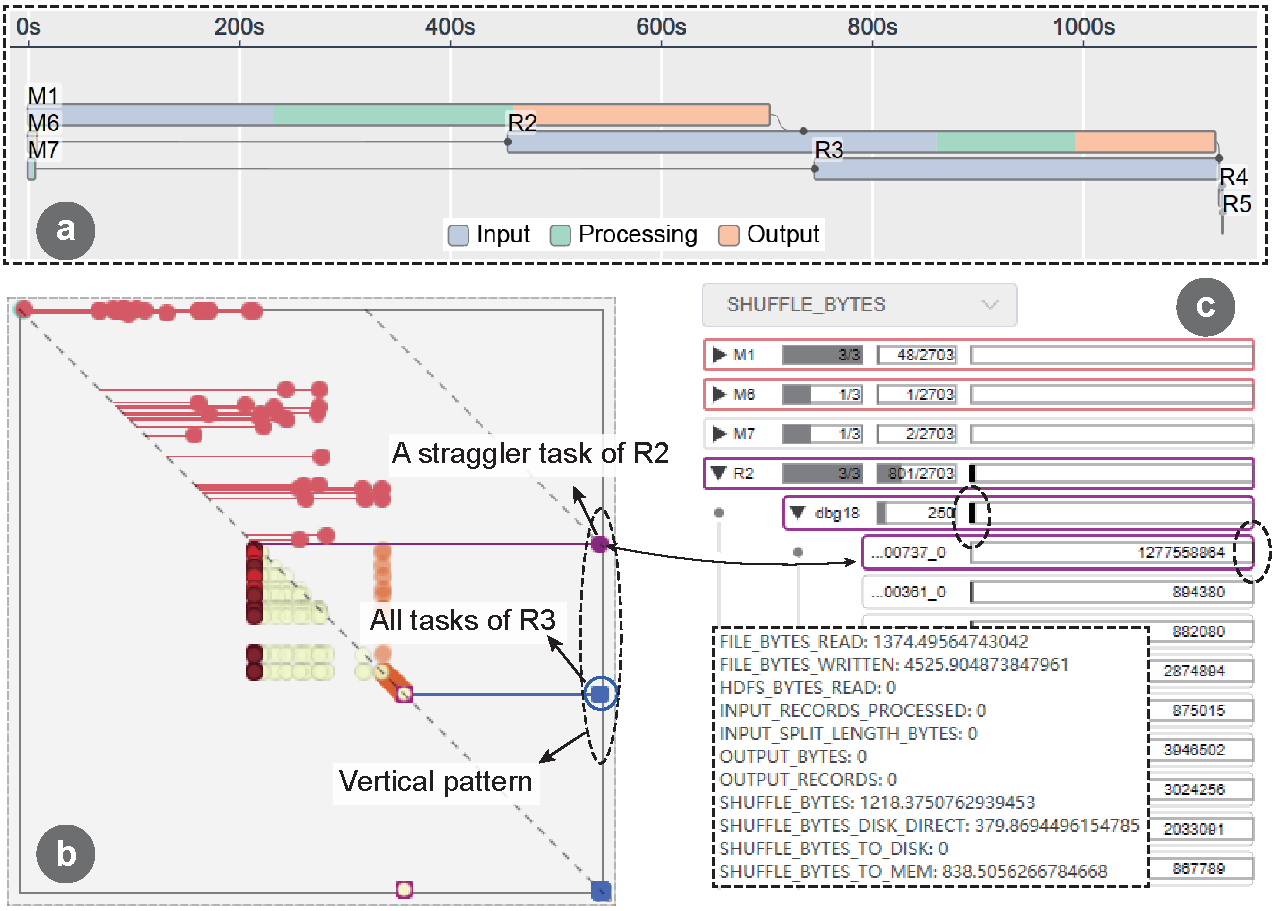
\includegraphics[width=0.46\textwidth]{figures/case_study/CaseStudy3SDS.pdf}
	\vspace{-2mm}
	\caption{\qevis{} detects data skew}
	\label{fig:casestudy3}
	\vspace{-5mm}
\end{figure}


\stitle{Step 1: identify performance bottleneck via \textit{job view}}
We inspect its \vtitle{job view} in \autoref{fig:casestudy3}(a) and observe that the input phase dominates the running time of job R3.
To find the reason for the long input time in job R3, we examine all its tasks via \vtitle{task view} in \autoref{fig:casestudy3}(b).


\stitle{Step 2: locate the straggler task via \textit{task view}}
We find that (i) all tasks of job R3 are concentrated in a small region, and (ii) there is a straggler task of job R2, which are highlighted in blue and purple circles in \autoref{fig:casestudy3}(b), respectively.
Moreover, there is a \textbf{vertical} execution pattern among the tasks of job R3 and the straggler task of job R2,
see the dashed eclipse, which suggests that the downstream tasks (of job R3) are waiting for the upstream task (of job R2).
%We next analyze the straggle task of job R2 via \vtitle{entity list}.

\stitle{Step 3: reason about the straggler task via \vtitle{entity list}}
By clicking the straggler task of job R2 in the \vtitle{task view}, the row of this task is automatically located and highlighted with a purple boundary in \autoref{fig:casestudy3}(c). 
We analyze its long running time by checking its processed data size, i.e., switching to ``SHUFFLE$\_$BYTES'' in the dropdown menu.
Surprisingly, the processed data volume of this straggler task is almost 1000 times of the other tasks in job R2, which indicates a severe data skew among the tasks.
Thus, the above unusually long running query is caused by data skew problem.

\qm{
	\stitle{Discussion} 
%	V1
%	In this case, multiple tasks exhibit abnormal execution behavior, but only one task, which suffers from data skewness, serves as the primary bottleneck for the entire execution process. Accurately identifying this specific bottleneck task necessitates the visualization of both tasks and their dependencies. This crucial visualization capability is provided exclusively by \qevis{}.
This case study highlights a scenario where a single task, experiencing data skewness, acts as the primary bottleneck in the execution process. Although multiple tasks exhibit abnormal execution behavior, correctly pinpointing this specific task is vital. This requires an intricate visualization of tasks along with their dependencies, a feature uniquely offered by \qevis{}.
}

%Through $\qevis$, we can conclude , then experienced engineers will try to alleviate it by re-configure the maximum number of task in Apache \hive{}. 

%\EVA{Can we show the optimization strategy?}



%\subsection{Case study} \label{sec:case}

%$\qevis{}$ has been deployed in the production environment of Huawei Cloud and is widely used by software engineers.
$\qevis{}$ has been deployed in the production environment and is widely used by software engineers.
Usually, our users are interested in queries that run longer than expected because they degrade system throughput. 
In this section, we demonstrate the effectiveness of \qevis{} via three use cases \qm{about slow query} in production, which identifies hardware, system and data problems during query execution, respectively.


\subsubsection{Identifying hardware problem} \label{sec:systemproblem}
\autoref{fig:teaser} shows how \qevis{} visualizes a long running query (i.e., 623 seconds) from a business intelligence application and we analyze it as follows.

\stitle{Step 1: investigate the performance bottleneck via \textit{job view}}
The \textit{job view} of the query is shown in \autoref{fig:teaser}(b).
Visually, job M1 has a very long running time.
More importantly, there is a large gray region in job M1, which means that the number of running tasks is 0 in this region according to the design of job rectangle in \autoref{sec:job}.
Thus, job M1 is the cause of long execution.


\stitle{Step 2: inspect job M1's task execution pattern via \textit{task view}}
To find the reasons that cause the gray region for job M1 in the \textit{job view}, we analyze the tasks of job M1 via the \textit{task view}.
When hovering the mouse on the job rectangle of M1, its associated tasks are highlighted with purple color in the \textit{task view}, see \autoref{fig:teaser}(d). 
We observe that the tasks of job M1 form two groups (i.e., \textbf{multi-cluster} pattern) that are far away from each other, as illustrated by the two dashed ellipses in \autoref{fig:teaser}(d). 
As discussed in \autoref{sec:task}, the multi-cluster pattern suggests that the tasks of job M1 are not executed properly due to machine problems.

\stitle{Step 3: locate the problematic machine via \textit{entity list}}
We know that the long running query is caused by machine problems but it is difficult to pinpoint the problematic machines as the production cluster is large.
Fortunately, \qevis{} provides the \textit{entity list} to map tasks to their executing machines.
By checking the \textit{entity list}, as illustrated by the rows with purple stroke in \autoref{fig:teaser}(e1), 
we observe that the tasks of job M1 in the right-bottom corner are executed on machine dbg18
%~\footnote{We anonymize the machine identifiers as required by our industry partner.}.
Then, we take a closer look at the tasks executed on dbg18, see \autoref{fig:teaser}(d1).
Compared with the other machines (e.g., dbg16, dbg19, dbg20), the number of tasks executed by dbg18 is quite small,
which suggests that the resource scheduler YARN allocates a small number of tasks to dbg18. 
This confirms that dbg18 is the problematic machine and YARN is aware of this fact during the query execution progress.
%With the conclusion above, we contact the infrastructure team and they confirm with us that the hard disk of dbg18 incurs errors.

Similar analyzing steps are also applied to job M24, which is another long running job in the query. 
We find that the long running time of job M24 is caused by a few straggling tasks on dbg19.
By investigating them, we find that dbg19 has high CPU utilization, see the red regions of the CPU usage heatmap in \autoref{fig:teaser}(f). 
We omit its analyzed steps as they are similar to the steps for job M1. 

To sum up, hardware problems cause the long running query. 
To verify, we remove dbg18 and dbg19, and re-run the query. The running time becomes 200 seconds.
\autoref{fig:teaser}(b1) shows the new \textit{job view}, where the running time of jobs M1 and M24 are much shorter than before.

\qm{
\stitle{Discussion}
%In this case study, the task cross-view linage and task level visualization analysis plays an important role in facilitate the execution exploration. Through the linkage among \vtitle{job view} and \vtitle{task view}, we quickly find the abnormal tasks (the group of late executed tasks) and then find these tasks are executed on a problematic machine which run very few tasks. 
%In this case study, the long execution of query is caused by multiple hardware problem, which is commonly appeared in real applications. The task level visualization of \qevis{} is key to facilitate exploration in this case. It allows users to quickly identify the abnormal tasks. Then we find their commonness through the cross-view linkage (\vtitle{task view} and \vtitle{entity list}), which is that all of these machines are executed on dbg18. Then we use \vtitle{task view} of dbg18 to confirm that the machine is suffering from hardware problem. 
%In this case study, the prolonged query execution is attributed to several hardware issues, a common occurrence in real-world applications. The task-level visualization provided by \qevis{} plays a crucial role in aiding exploration in this particular case. It enables users to promptly identify abnormal tasks. Through cross-view linkage, specifically between the task view and entity list, we determine a common factor: all these tasks are executed on dbg18. Further utilizing the task view of dbg18, we confirm that the machine is indeed experiencing a hardware problem.
%In this case study, the query execution suffers from multiple hardware issues. The \vtitle{task view} of all tasks plays a crucial role in aiding exploration by enabling users to promptly identify the abnormal tasks. The \vtitle{task view} of dbg18 further shows that the machine dbg18 which executes the abnormal tasks is suffering from a hardware problem.
%
%The \vtitle{task view} offered by \qevis{} plays a crucial role in aiding exploration by enabling users to promptly identify the abnormal tasks.  Then we confirm these tasks are executed on the same machine dbg18 through the linkage between \vtitle{task view} and \vtitle{entity list}, and inspect taht this machine is indeed experiencing a hardware problem. 
In this case study, the query execution suffers from multiple hardware issues. The \vtitle{task view} of all tasks plays a crucial role by quickly identifying abnormal tasks. Furthermore, the \vtitle{task view} of dbg18 further shows that the machine dbg18 which executes the abnormal tasks is suffering from a hardware problem. This scenario demonstrates that the visual pattern of tasks is helpful in diagnosing these issues efficiently.
}

\subsubsection{Identifying system problem}
We analyze a query that generates app downloads report for market analysis in this case.
\begin{figure}
	\centering
	\small
	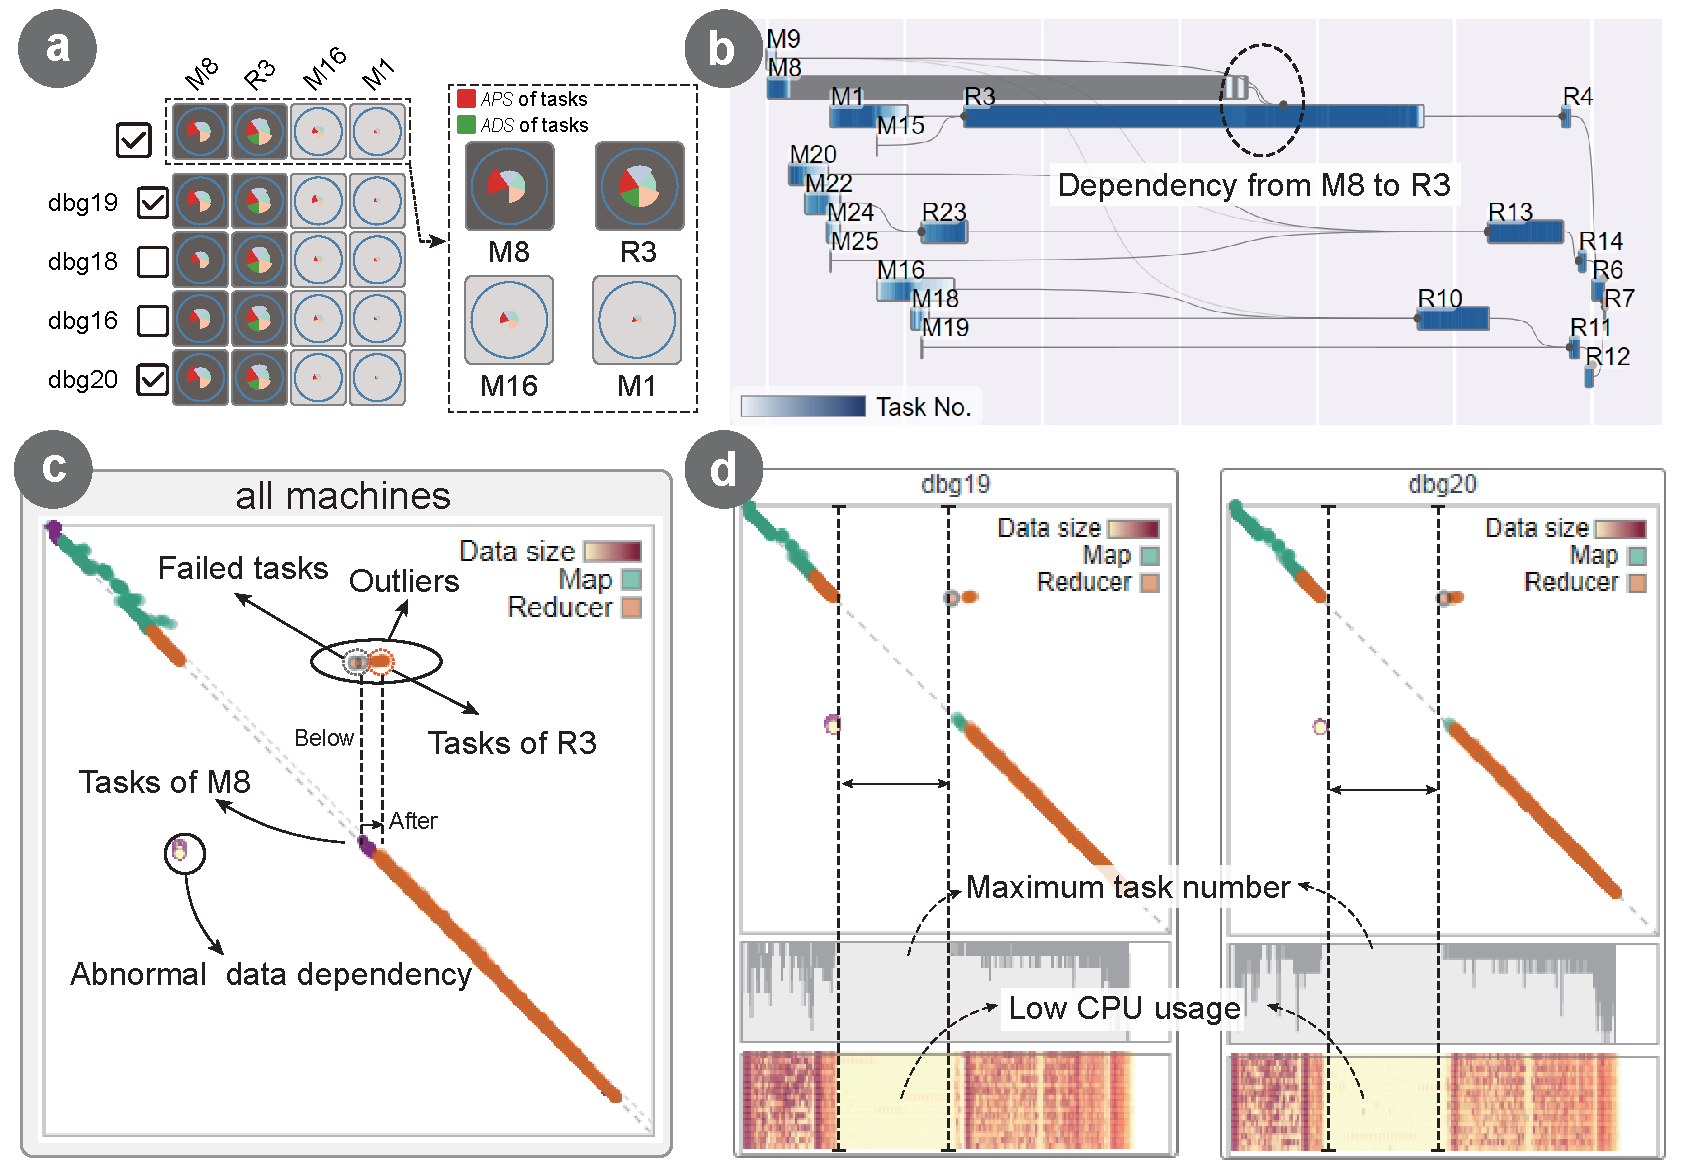
\includegraphics[width=0.46\textwidth]{figures/case_study/CaseStudy2SDS.pdf}  
	\vspace{-3mm}
	\caption{\qevis{} identifies system problem (task deadlock)} 
	\label{fig:casestudy2}
	\vspace{-5mm}
\end{figure}

\stitle{Step 1: observe abnormal jobs via \vtitle{performance matrix}}
As shown by the \textit{performance matrix} in \autoref{fig:casestudy2}(a), the anomaly scores of jobs R3 and M8 are significantly larger than the other jobs, especially the abnormal duration scores (i.e., red sectors). 
Moreover, the green sector (i.e., abnormal parallelism score) of job R3 is also very large.
Since job R3 is the downstream job of M8 as shown in the \textit{job view} in \autoref{fig:casestudy2}(b), 
we conjecture that there is a causal relation between the abnormal behaviors of jobs M8 and R3.


\stitle{Step 2: reveal abnormal data dependency via \vtitle{task view}}
We next perform fine-grained exploration on the tasks via the \vtitle{task view}.
There are several \textbf{outliers}, as highlighted in \autoref{fig:casestudy2}(c).
These outlier tasks can be classified into two categories: (i) failed tasks (the gray points), and (ii) long running tasks (highlighted in orange color).
Interestingly, several tasks of map job M8 are executed immediately after these failed tasks, and then the orange colored tasks of reducer job R3 are executed.
Visually, we can see there are several purple points (i.e., the tasks of job M8) vertically located below the gray points (i.e., failed tasks) and the orange points (i.e., tasks of job R3) are horizontally located after the purple points.
Thus, we confirm that there are abnormal data dependencies among the tasks of jobs M8 and R3, shown as the data dependency points in the left-bottom part of \autoref{fig:casestudy2}(c).


\stitle{Step 3: reason about the failed tasks via \vtitle{profiling view}}
As the \vtitle{profiling view} of the machine is aligned with \vtitle{task view} by time, 
we observe that both dbg19 and dbg20 run the maximum number of tasks during the execution period of these failed tasks, see the range between the two vertical dashed lines for dbg 19 and dbg20 in \autoref{fig:casestudy2}(d). 
However, the CPU utilization of two machines is very low in this period. 
This suggests that the containers of the two machines are fully occupied but no work is done, and thus there is a task deadlock.
In particular, the resource scheduler YARN assigns all containers of dbg19 and dbg20 to the tasks of job R3, and these tasks are waiting for the input data from the upstream tasks of job M8. But the upstream tasks cannot be executed as there are no idle containers, and thus the tasks of jobs M8 and R3 form a circular waiting.
The deadlock is resolved after killing several tasks of job R3, as depicted by the gray colored failed tasks in \autoref{fig:casestudy2}(c).

\qm{
	\stitle{Discussion} 
%	The deadlock appears when the computing resource is limited and too much containers are allocated by source manager(e.g., Yarn). \qevis{} can help analysts identify the deadlock cases with following features: by employing task level visualization with dependencies and properly aligning the timing information of tasks and system profiling.
%Deadlocks occur when computing resources are scarce and an excessive number of containers are allocated by the resource manager (e.g., Yarn). \qevis{} assist analysts to identify deadlock cases through the following features: task-level visualization incorporating dependencies and accurate alignment of timing information from tasks and system profiling. These capabilities enable analysts to gain insights into deadlock situations effectively.
%Deadlocks occur when computing resources are scarce and an excessive number of containers are allocated by the resource manager (e.g., Yarn). \qevis{} assist analysts to identify deadlock cases through the following features: task-level visualization incorporating dependencies and accurate alignment of timing information from tasks and system profiling. These capabilities enable analysts to gain insights into deadlock situations effectively.
%V1
%Deadlocks occur when there's a shortage of computing resources and the resource manager (e.g., Yarn) over-allocates containers. \qevis{} brings following features to address such scenarios: it represents task distribution, enabling users to swiftly identify critical tasks; it displays dependencies that indicate logical relationships among tasks; and it aligns system profiling with execution patterns to illustrate the interplay between resources and execution. The conventional approaches may struggle to manage this situation due to their lack of task oriented visaulization (both task and dependency) and task-system profiling alignment.
%V2
Deadlocks occur when there is a shortage of computing resources and suboptimal task scheduling by resource managers (e.g., Yarn). \qevis{} addresses this by offering following key features: task distribution for quick identification of critical tasks, dependency visualization for understanding logical task relationships and alignment of execution patterns with system profiling to show the interplay between resources and execution. The conventional approaches may struggle to manage this situation due to their lack of task oriented visualization (both task and dependency) and task-system profiling alignment.
}
\subsubsection{Identifying data problem}
We next analyze a query that runs daily for sales analysis, which takes 1200 seconds and is longer than before. 

\begin{figure}[t]
	\centering
	\small
	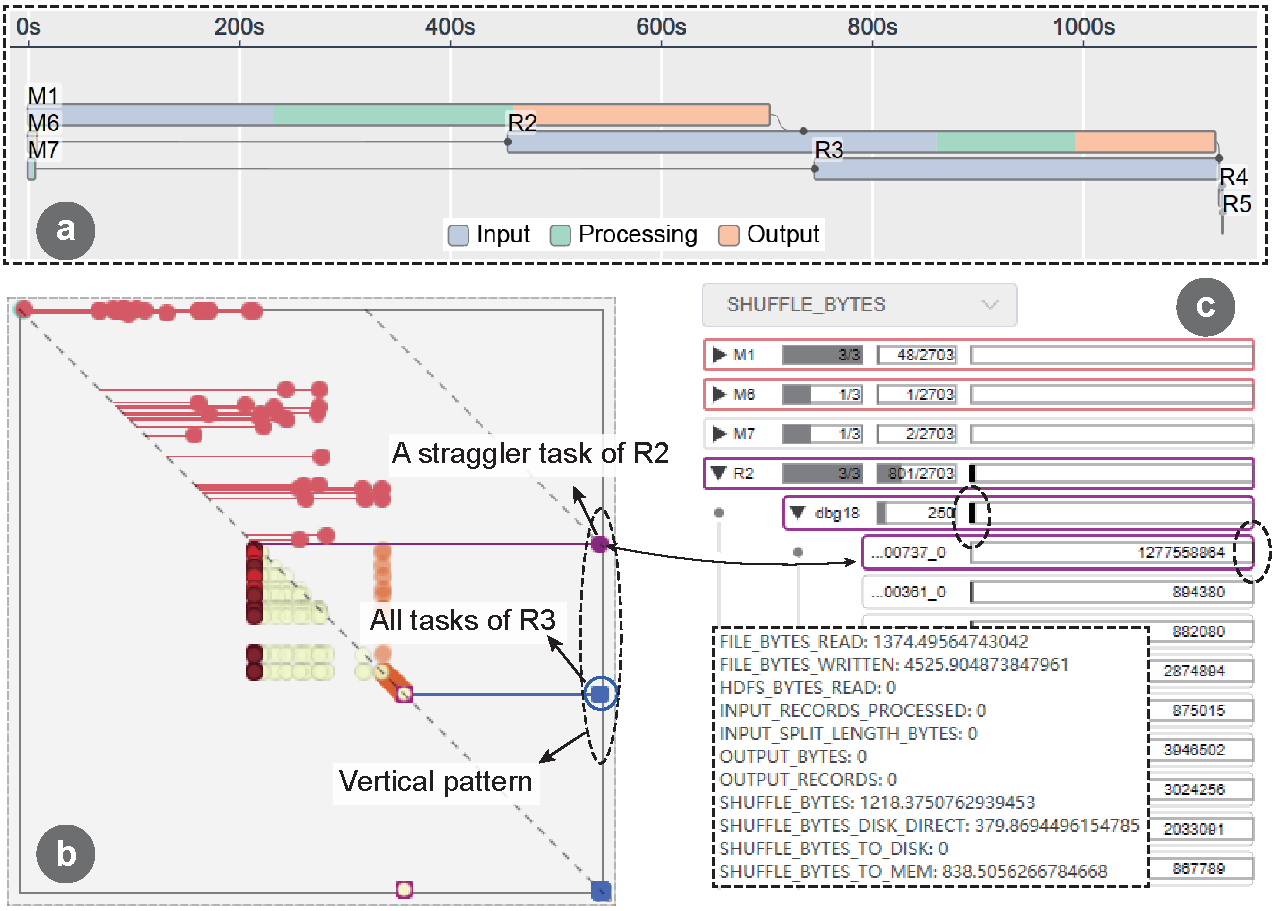
\includegraphics[width=0.46\textwidth]{figures/case_study/CaseStudy3SDS.pdf}
	\vspace{-2mm}
	\caption{\qevis{} detects data skew}
	\label{fig:casestudy3}
	\vspace{-5mm}
\end{figure}


\stitle{Step 1: identify performance bottleneck via \textit{job view}}
We inspect its \vtitle{job view} in \autoref{fig:casestudy3}(a) and observe that the input phase dominates the running time of job R3.
To find the reason for the long input time in job R3, we examine all its tasks via \vtitle{task view} in \autoref{fig:casestudy3}(b).


\stitle{Step 2: locate the straggler task via \textit{task view}}
We find that (i) all tasks of job R3 are concentrated in a small region, and (ii) there is a straggler task of job R2, which are highlighted in blue and purple circles in \autoref{fig:casestudy3}(b), respectively.
Moreover, there is a \textbf{vertical} execution pattern among the tasks of job R3 and the straggler task of job R2,
see the dashed eclipse, which suggests that the downstream tasks (of job R3) are waiting for the upstream task (of job R2).
%We next analyze the straggle task of job R2 via \vtitle{entity list}.

\stitle{Step 3: reason about the straggler task via \vtitle{entity list}}
By clicking the straggler task of job R2 in the \vtitle{task view}, the row of this task is automatically located and highlighted with a purple boundary in \autoref{fig:casestudy3}(c). 
We analyze its long running time by checking its processed data size, i.e., switching to ``SHUFFLE$\_$BYTES'' in the dropdown menu.
Surprisingly, the processed data volume of this straggler task is almost 1000 times of the other tasks in job R2, which indicates a severe data skew among the tasks.
Thus, the above unusually long running query is caused by data skew problem.

\qm{
	\stitle{Discussion} 
%	V1
%	In this case, multiple tasks exhibit abnormal execution behavior, but only one task, which suffers from data skewness, serves as the primary bottleneck for the entire execution process. Accurately identifying this specific bottleneck task necessitates the visualization of both tasks and their dependencies. This crucial visualization capability is provided exclusively by \qevis{}.
This case study highlights a scenario where a single task, experiencing data skewness, acts as the primary bottleneck in the execution process. Although multiple tasks exhibit abnormal execution behavior, correctly pinpointing this specific task is vital. This requires an intricate visualization of tasks along with their dependencies, a feature uniquely offered by \qevis{}.
}

%Through $\qevis$, we can conclude , then experienced engineers will try to alleviate it by re-configure the maximum number of task in Apache \hive{}. 

%\EVA{Can we show the optimization strategy?}



%\input{5.1_case}


%However, there is a straggler task, which incurs significantly long running time, 
%We find that the tasks of job R3 are all concentrated in a very small region (shown as \autoref{fig:casestudy3}(b2)) but an abnormal task runs significantly longer than the other tasks (shown as \autoref{fig:casestudy3}(b1)). 
%When hovering the mouse on task b1, we find that all tasks of R3 are colored blue, which means that task b1 was the provider for all tasks of R3 and the tasks of R3 are delayed because they are waiting for b1. After task b1 finishes, the entire query finishes almost immediately, suggesting that task b1 is the bottleneck of the query.



%one task of M24 runs for a long time on machine dbg19. Moreover, he also found a more obvious \textbf{dispersion pattern} in the \vtitle{task view} of dbg19 than the other machines, which indicates dbg19 is suffering from problem.







%The query is executed on a cluster with five machines (shown in \autoref{fig:teaser}(a)) and runs for about 623 seconds, which is much longer than usual. Thus, E1 used \qevis{} to find the reasons. 


%E1 started his exploration from the overview of query execution, i.e., \textit{job view} shown in \autoref{fig:teaser}(b). 
%phase 1 overview
%He found that job M1 had a significantly longer duration than the other jobs and had a long grey region indicating no tasks of M1 were executed during this period. Moreover, R2, a job consumed M1, finished quickly after M1 was completed, and the same applied to other reducer jobs (R3-6, 8, 10, 11) according to \autoref{fig:teaser}(b). 
%Thus, he inspected that M1 may be the performance bottleneck leading to the long execution time of this query.
% phase 2 detail view
%Then he hovered the mouse on M1 to highlight the associated tasks with purple color in the \vtitle{task view} shown as \autoref{fig:teaser}(d). 
%He observed that M1's tasks formed two groups far away from each other (\textbf{multi-cluster pattern}), as shown in the dashed ellipses in \autoref{fig:teaser}(d). 
%By checking the \vtitle{entity list} (shown as the rows with purple stroke in \autoref{fig:teaser}(e1)), he found that the tasks in the right-bottom corner were only executed on machine dbg18 since all the tasks executing on other machines finished much early.
%When observing the \vtitle{task view} of dbg18, he found dbg18 executed far fewer tasks than the other machines shown as \autoref{fig:teaser}(d1), which suggested that dbg18 may have internal problems. After checking the system log, he found that something was wrong with the network of dbg18, which caused the resource manager to allocate a small number of tasks to it and the late execution of these tasks. 

% phase 1, overview 
%Besides M1, he noticed that another Map job, M24, also had a long duration. By hovering the mouse on M24 to highlight its tasks, he found that none of them were executed on dbg18, and thus dbg18 was not the only performance bottleneck. 
% phase 2, detailed view
%In the \vtitle{task view}, he observed that one task of M24 runs for a long time on machine dbg19. Moreover, he also found a more obvious \textbf{dispersion pattern} in the \vtitle{task view} of dbg19 than the other machines, which indicates dbg19 is suffering from problem.
% phase 3, profiling view
%When exploring the system usage through \vtitle{profiling view}, he found that the CPU usage heatmap of dbg19 has large red regions, as shown in \autoref{fig:teaser}(f), indicating high CPU utilization. After a check, he found that several computation-intensive programs were also executed on dbg19 when running the query, resulting in resource contention.

%To address the identified problems, we remove machine dbg18 and kill the computation-intensive programs on machine dbg19. The query finishes within 200s this time. In the \textit{progress view}, we observe that the duration of both vertex M1 and M24 are much shorter than before, as shown in \autoref{fig:teaser}(B3). 
%We also find that all tasks are close to the diagonal line in the \textit{task distribution} in \autoref{fig:teaser}(D4)(\textbf{line parallel to diagonal} pattern in section~\ref{sec:taskdistribution}), indicating that they all have a short duration (thus no straggling task). 
%We also find that all tasks are close to the diagonal line in the \textit{task distribution} in \autoref{fig:teaser}(D4)(\textbf{line parallel to diagonal} pattern in section~\ref{sec:taskdistribution}), which is different from the previous \textbf{dispersion pattern}.





%\subsubsection{Reason task failure}




%The second query serves the purpose of generating a sales report sheet for the most recent two weeks. 
%It was run on a cluster with eight machines and was significantly slower than the last execution.
% \textcolor{red}{need to discribe the problem, to keep the same structure as 4.1}


%To further analyze the anomaly, we perform fine-grained exploration with the \vtitle{task view}.
%As dbg19 and dbg20 have significantly larger abnormal parallelism scores than the other machines (the red sector is larger), we inspect the \vtitle{task view} of all tasks (shown as \autoref{fig:casestudy2}(c)) and the \vtitle{task view} of these two machines (shown as \autoref{fig:casestudy2}(d)).
%From \autoref{fig:casestudy2}(c), we observe that most tasks are located close to the diagonal line, which is the \textbf{parallel pattern} (see Section~\ref{sec:task}) and indicates that they are  executed smoothly. However, there are several outliers in \autoref{fig:casestudy2}(c2), which is the \textbf{outlier pattern} and indicates that these tasks take much longer time than normal. Moreover, there are two failed tasks in these outliers (marked with grey boundaries). 
% \autoref{fig:casestudy2}(c) shows that most tasks were located close to the diagonal line (\textbf{parallel pattern}) while several outliers (\textbf{outlier pattern}) of R3 were far from the diagonal line, which is shown as \autoref{fig:casestudy2}(c2). 
% In addition, two of these tasks fail (marked with grey boundaries) and we want to know why. 

%\stitle{Step 3: }
%Now, we combine the \vtitle{task view} and \vtitle{profiling view} to find the causes of the failed tasks. 
%\vtitle{Task view} shows that the two failed tasks are executed on dbg19 and dbg20, respectively.
%As the \vtitle{profiling view} is aligned with \vtitle{task view} by time, we can observe that both dbg19 and dbg20 run the maximum number of tasks during the execution period of the two failed tasks (see the range marked by the two vertical dashed lines in \autoref{fig:casestudy2}(d1, d2)). 
%However, the CPU utilization of the two machines is low until the two tasks fail. This suggests that all containers of these two machines are occupied but these containers do not conduct work until the two tasks are killed. 
%Moreover, by hovering the mouse on the points in \autoref{fig:casestudy2}(c3), we observe that there are abnormal dependencies from tasks c1 to c2 in \autoref{fig:casestudy2}(c), indicating that job R3's task c2 is waiting for job M8's task c1.

%The observations above make us conjecture that the two tasks of R3 fail because of resource deadlock---job R3's task c2 waits for input from job M8's task c1 but all containers in dbg19 and dbg20 are occupied, and thus task c1 can not be scheduled, which blocks task c2 and prevents it from releasing the container. The system handles this deadlock by killing the two tasks of R3 on dbg19 and dbg20 to leave containers to execute M8's task c1, and R3's tasks finish quickly after receiving input data. 


%However, there is a straggler task, which incurs significantly long running time, 
%We find that the tasks of job R3 are all concentrated in a very small region (shown as \autoref{fig:casestudy3}(b2)) but an abnormal task runs significantly longer than the other tasks (shown as \autoref{fig:casestudy3}(b1)). 
%When hovering the mouse on task b1, we find that all tasks of R3 are colored blue, which means that task b1 was the provider for all tasks of R3 and the tasks of R3 are delayed because they are waiting for b1. After task b1 finishes, the entire query finishes almost immediately, suggesting that task b1 is the bottleneck of the query.



%one task of M24 runs for a long time on machine dbg19. Moreover, he also found a more obvious \textbf{dispersion pattern} in the \vtitle{task view} of dbg19 than the other machines, which indicates dbg19 is suffering from problem.







%The query is executed on a cluster with five machines (shown in \autoref{fig:teaser}(a)) and runs for about 623 seconds, which is much longer than usual. Thus, E1 used \qevis{} to find the reasons. 


%E1 started his exploration from the overview of query execution, i.e., \textit{job view} shown in \autoref{fig:teaser}(b). 
%phase 1 overview
%He found that job M1 had a significantly longer duration than the other jobs and had a long grey region indicating no tasks of M1 were executed during this period. Moreover, R2, a job consumed M1, finished quickly after M1 was completed, and the same applied to other reducer jobs (R3-6, 8, 10, 11) according to \autoref{fig:teaser}(b). 
%Thus, he inspected that M1 may be the performance bottleneck leading to the long execution time of this query.
% phase 2 detail view
%Then he hovered the mouse on M1 to highlight the associated tasks with purple color in the \vtitle{task view} shown as \autoref{fig:teaser}(d). 
%He observed that M1's tasks formed two groups far away from each other (\textbf{multi-cluster pattern}), as shown in the dashed ellipses in \autoref{fig:teaser}(d). 
%By checking the \vtitle{entity list} (shown as the rows with purple stroke in \autoref{fig:teaser}(e1)), he found that the tasks in the right-bottom corner were only executed on machine dbg18 since all the tasks executing on other machines finished much early.
%When observing the \vtitle{task view} of dbg18, he found dbg18 executed far fewer tasks than the other machines shown as \autoref{fig:teaser}(d1), which suggested that dbg18 may have internal problems. After checking the system log, he found that something was wrong with the network of dbg18, which caused the resource manager to allocate a small number of tasks to it and the late execution of these tasks. 

% phase 1, overview 
%Besides M1, he noticed that another Map job, M24, also had a long duration. By hovering the mouse on M24 to highlight its tasks, he found that none of them were executed on dbg18, and thus dbg18 was not the only performance bottleneck. 
% phase 2, detailed view
%In the \vtitle{task view}, he observed that one task of M24 runs for a long time on machine dbg19. Moreover, he also found a more obvious \textbf{dispersion pattern} in the \vtitle{task view} of dbg19 than the other machines, which indicates dbg19 is suffering from problem.
% phase 3, profiling view
%When exploring the system usage through \vtitle{profiling view}, he found that the CPU usage heatmap of dbg19 has large red regions, as shown in \autoref{fig:teaser}(f), indicating high CPU utilization. After a check, he found that several computation-intensive programs were also executed on dbg19 when running the query, resulting in resource contention.

%To address the identified problems, we remove machine dbg18 and kill the computation-intensive programs on machine dbg19. The query finishes within 200s this time. In the \textit{progress view}, we observe that the duration of both vertex M1 and M24 are much shorter than before, as shown in \autoref{fig:teaser}(B3). 
%We also find that all tasks are close to the diagonal line in the \textit{task distribution} in \autoref{fig:teaser}(D4)(\textbf{line parallel to diagonal} pattern in section~\ref{sec:taskdistribution}), indicating that they all have a short duration (thus no straggling task). 
%We also find that all tasks are close to the diagonal line in the \textit{task distribution} in \autoref{fig:teaser}(D4)(\textbf{line parallel to diagonal} pattern in section~\ref{sec:taskdistribution}), which is different from the previous \textbf{dispersion pattern}.





%\subsubsection{Reason task failure}




%The second query serves the purpose of generating a sales report sheet for the most recent two weeks. 
%It was run on a cluster with eight machines and was significantly slower than the last execution.
% \textcolor{red}{need to discribe the problem, to keep the same structure as 4.1}


%To further analyze the anomaly, we perform fine-grained exploration with the \vtitle{task view}.
%As dbg19 and dbg20 have significantly larger abnormal parallelism scores than the other machines (the red sector is larger), we inspect the \vtitle{task view} of all tasks (shown as \autoref{fig:casestudy2}(c)) and the \vtitle{task view} of these two machines (shown as \autoref{fig:casestudy2}(d)).
%From \autoref{fig:casestudy2}(c), we observe that most tasks are located close to the diagonal line, which is the \textbf{parallel pattern} (see Section~\ref{sec:task}) and indicates that they are  executed smoothly. However, there are several outliers in \autoref{fig:casestudy2}(c2), which is the \textbf{outlier pattern} and indicates that these tasks take much longer time than normal. Moreover, there are two failed tasks in these outliers (marked with grey boundaries). 
% \autoref{fig:casestudy2}(c) shows that most tasks were located close to the diagonal line (\textbf{parallel pattern}) while several outliers (\textbf{outlier pattern}) of R3 were far from the diagonal line, which is shown as \autoref{fig:casestudy2}(c2). 
% In addition, two of these tasks fail (marked with grey boundaries) and we want to know why. 

%\stitle{Step 3: }
%Now, we combine the \vtitle{task view} and \vtitle{profiling view} to find the causes of the failed tasks. 
%\vtitle{Task view} shows that the two failed tasks are executed on dbg19 and dbg20, respectively.
%As the \vtitle{profiling view} is aligned with \vtitle{task view} by time, we can observe that both dbg19 and dbg20 run the maximum number of tasks during the execution period of the two failed tasks (see the range marked by the two vertical dashed lines in \autoref{fig:casestudy2}(d1, d2)). 
%However, the CPU utilization of the two machines is low until the two tasks fail. This suggests that all containers of these two machines are occupied but these containers do not conduct work until the two tasks are killed. 
%Moreover, by hovering the mouse on the points in \autoref{fig:casestudy2}(c3), we observe that there are abnormal dependencies from tasks c1 to c2 in \autoref{fig:casestudy2}(c), indicating that job R3's task c2 is waiting for job M8's task c1.

%The observations above make us conjecture that the two tasks of R3 fail because of resource deadlock---job R3's task c2 waits for input from job M8's task c1 but all containers in dbg19 and dbg20 are occupied, and thus task c1 can not be scheduled, which blocks task c2 and prevents it from releasing the container. The system handles this deadlock by killing the two tasks of R3 on dbg19 and dbg20 to leave containers to execute M8's task c1, and R3's tasks finish quickly after receiving input data. 
\subsection{User Interview} \label{sec:user}

In this section, we discuss the feedback from the users of \qevis{}. 

\subsubsection{Feedback from long term collaborators}
The first set of feedback comes from our two long-term collaborators (i.e., P1 and P2), who helped formulate the design requirements and tasks of \qevis{} in ~\autoref{sec:qevisgoals}. The two experts collaborated with us for more than one year to build and improve \qevis{}. We conducted semi-structured interviews with them face to face and asked them to evaluate \qevis{} according to the design tasks. 

\stitle{Multi-scale visualization}
Both P1 and P2 agree that the multi-scale visualization of \qevis{} helps analysts conduct  a wide range of query execution analysis tasks. P2 comments that the design of the \vtitle{job view} is effective for the overview of query execution. He said ``the \vtitle{job view} is like a portrait and enables me to quickly comprehend the overall execution process of a query, which is particularly important when the same query is executed repetitively.'' P1 points out that the visual encoding of task parallelism and sub-phase percentage is helpful for users to determine whether a job is executed properly. Both P1 and P2 are satisfied with the scatter plot-based design of the \vtitle{task view} as it shows representative distribution patterns. P1 said that ``it provides a new visual form for analysts to quickly evaluate query execution and select the tasks of interest''. However, both P1 and P2 expect more flexible interactions such as selecting a group of tasks by drawing a polygon and visualizing the common feature of the selected tasks.

\stitle{Anomaly scoring and visualization}
Both P1 and P2 think that to measure the anomaly degree of jobs and machines, our general scoring methods are favorable. P1 suggests that the \vtitle{performance matrix} complements the \vtitle{job view} when the \vtitle{job view} does not provide clear clue for the component to inspect. P2 claims that he always starts his exploration from the \vtitle{performance matrix}, which also provides an overview of query execution. 
In addition, P2 recommends developing an anomaly score for the entire query, which provides a high-level summary of query execution and facilitates comparison between repetitive executions of the same or different queries.

\stitle{Enable pattern reasoning}
P1 and P2 think that the three-level design in the \vtitle{entity list} is useful,  especially when using multi-grained visualizations to explain the tasks with abnormal timing patterns. 
They also said that visually correlating system profiling with task execution helps explain abnormal task execution. However, P1 commented that the \vtitle{task view} and \vtitle{profiling view} are too small to inspect. He suggested allowing the users to extend the \vtitle{task view} and \vtitle{profiling view} to a large separate view when necessary.  

\subsubsection{Feedback from potential users}

\stitle{Settings}
\qm{The second set of interviews was conducted with six developers and engineers (E1-E6) in a company to evaluate the usability of \qevis{}. None of these participants used \qevis{} before the study. We provided them with 10 real-world application cases, specifically chosen from applications with extended execution times. These executions exhibited various issues such as insufficient resources, incorrect configuration, and hardware problems. Participants were instructed to freely explore these cases with \qevis{} and draw conclusions regarding the factors contributing to the slow query executions. 
The study was conducted on a screen with a resolution of 1980 x 1080, and each session lasted 80 minutes, including a 5-minute demonstration video, a 5-minute introduction to the study, a 15-minute introduction to \qevis{}, and 55 minutes for free exploration.
During the study, the participants were encouraged to think aloud, allowing us to collect feedback in real time. 
After the study, they were asked to fill out a questionnaire with seven questions, which are listed as follows:
}

\squishlist
\item[\textbf{Q1}] Which view is the most important during your exploration? 
\item[\textbf{Q2}] Which view do you use the most during your exploration?
\item[\textbf{Q3}] How does \qevis{} compare to similar tools you have used?
\item[\textbf{Q4}] How easy is it to learn to use \qevis{}? 
\item[\textbf{Q5}] How easy is it to navigate and find what you need?
\item[\textbf{Q6}] Do you have any other comments or suggestions?
\squishend

For \textbf{Q4} and \textbf{Q5}, the participants can rate the difficulty level on a scale from 1 to 7, with 1 indicating "very difficult" and 7 indicating ``very easy''. We also encouraged the participants to write down the reasons for their answers. 

\stitle{Feedback discussion} 
Regarding \textbf{Q1}, 4 out of the 6 participants identified the \vtitle{task view} as the most important during their exploration. They noted that they needed to use this view to find the root causes of query execution anomalies. E1 selected the \vtitle{job view} and said that he could inspect query execution by switching among different modes. E6 selected the \vtitle{performance matrix} because it indicates the problematic machines.

In response to \textbf{Q2}, 4 out of the 6 participants also selected the \vtitle{task view} as the most used view because they spent a lot of time switching between the \vtitle{task view} and \vtitle{entity list} to find the causes of long-running tasks. The \vtitle{job view} and \vtitle{entity list} were also selected by one participant.

Regarding \textbf{Q3}, only E1 has not used other query visualization tools before. E2-5 were familiar with TezUI, while E2 and E6 had experience with Dr. Elephant. 
E2 and E3 commented that \qevis{} was more flexible than TezUI due to its interactions and cross-view linkage. ``It can help me to quickly identify the execution pattern of the tasks in a job'', claimed by E2. E3 stated that the \vtitle{job view} helped him quickly compare different executions of the same query and he did not need to switch between different web pages.
E6 thought that \qevis{} was harder to use than the automatic query diagnosis in Dr. Elephant but agreed that \qevis{} is more powerful in analyzing complex execution problems. He suggested integrating more algorithms to measure the anomaly degree of machines based on profiling and correlate machine anomalies with task execution.

In response to \textbf{Q4}, the participants gave an average score of 5.6, with a minimum score of 3 and a maximum score of 7. Participants that have used other visualization tools tended to be more positive about \qevis{} (E2-5). 
However, E6, who gave the minimum score, commented that there were too many visual channels (e.g., color encoding, size, shape) in \qevis{} and it is hard to remember them. He suggested adding more detailed legends to explain the meaning of the visual encodings.  


Regarding navigation (\textbf{Q5}), the participants gave an average score of 6, with a minimum score of 5 and a maximum score of 7. The participants stated that the cross-view linkage made it easy to find the elements of interest. 


In summary, the user study suggests that \qevis{} is a powerful and user-friendly tool for diagnosing runtime anomalies in distributed query execution, although there is still room for improvement.

%E6 suggested integrating more powerful algorithms to measure the anomaly degree of machines based on profiling and correlating the machine anomaly with runtime behavior. Moreover, E2 and E3 encouraged designing a more flexible framework that allows users to choose which view to display because they found that not all views are used during each exploration.



\section{Discussions and lessons learned} \label{sec:discussion}

In this part, we discuss the lessons learned from the \qevis{} project.

\stitle{Collaboration}
%Effectively collaborating with domain experts is important. Long-term observation of how domain experts solve their problem in real scenarios is necessary to understand and extract their requirements, specifically, the visualization researchers are also encouraged to participate in the work of domain experts. Moreover, we also encourage involving some of the domain experts in the visualization design. For example, when selecting coordinate encoding in the dependency distribution view, the domain experts suggest visualizing the abnormal dependencies in the left bottom part to make better use of the canvas and effectively reveal the information that should be attentioned.  
Effective collaboration with domain experts is crucial for the designs of the domain-specialized visualizations in \qevis{}. Close observations of how they solve problems in real scenarios are key to understanding and summarizing the design requirements. Visualization researchers should participate in or at least try the work of domain experts, and conversely domain experts should be encouraged to give suggestions to visual designs. For example, when selecting coordinate encoding in the \vtitle{dependency distribution}, the domain experts suggested visualizing the abnormal dependencies in the left bottom part to make better use of the canvas and effectively reveal the information that is worth paying attention to.


\stitle{Overview vs. detail view}
Choosing the right analysis granularity is important for solving specific tasks. Logical plan visualization (\vtitle{job view}) is easy to understand and can help solve high-level problems. Atomic task visualization (\vtitle{task view}), on the other hand, contains many tasks that are executed distributedly and is more difficult to understand. However, it is usually necessary for solving low-level problems such as query debugging and execution bottleneck identification. 
We recommend that the users choose different visualization granularities on demand. 
For instance, novice users can start with logical level visualization for a general understanding of the query execution process and narrow their exploration progressively, while experienced users can directly begin with the \vtitle{task view} for in-depth analysis.



\stitle{Generalization}
%One important consideration of \qevis{} is to generalize across different distributed query execution systems. 
%We observe that these systems adopt a similar query processing procedure --- a query is first transformed into a logical plan and then into a physical plan, which is mapped to task/operator instances on the machines for execution. The logical/physical plans usually take the form of DAG or tree. By designing visualizations for temporal DAG (with tree being a special case of DAG) and handling many physical instances (i.e., tasks), \qevis{} has the potential to work with distributed systems other than Hive, which we left as future work.    
%Even the current system is designed based on \hive{}, the architecture and visualization design can be easily applied to other distributed query execution in which the logical plan can be modeled as DAG. 
%Different systems (e.g., Hive, Spark, Flink) are used for different workloads (e.g., bulk processing, stream processing, and in-memory analytics). 
%Although \qevis{} was mainly designed for \hive{}, it can be easily extended to other distributed query processing systems (e.g., Spark and Flink) because these systems share many common features. For instance, the logical query plan can be modeled as a directed acyclic graph (DAG) of jobs, and the tasks of a job are executed on the machines in parallel. Thus, the visual designs of \qevis{} can generalize across different systems.  
\qm{
%Although \qevis{} was mainly designed for \hive{}, its key components can be widely extended to other distributed query processing systems and parallel computing systems which employ the directed acyclic graph (DAG) as their computational abstractions, such as Spark, Flink,  AsterixDB, Impala, SCOPE and Myria. However, the users should also pay attention to the detailed difference bewteen Hive and other systems. For instance, when implementing \vtitle{task view} for Spark. The users should know that the tasks of Spark is that there is no waiting among the tasks because the comsumer tasks is scheduled after all the provider tasks are finished. THus, when visualizing the dependencies, the researchers should modify the visual design by switch the axis of depndencies.
While \qevis{} was primarily developed for \hive{}, its core components can be broadly applied to various distributed query  systems and parallel computing platforms that utilize the Directed Acyclic Graph (DAG) as their computational paradigm. These systems include, but are not limited to, Spark, Flink, AsterixDB~\cite{alsubaiee2014asterixdb}, Impala~\cite{bittorf2015impala}, SCOPE~\cite{chaiken2008scope}, and Myria. However, it's important for users to recognize and accommodate the subtle differences between \hive{} and the other systems. 
%Take, for instance, the implementation of a task view for Spark. 
Using Spark as an example, it is important for users to be aware that Spark's tasks are structured in such a way that there is no inter-task waiting, since consumer tasks are scheduled only after all the provider tasks have been completed. Therefore, when illustrating dependencies, researchers will need to adapt their visual design strategy, specifically by altering the axis of dependencies.
}

%the query systems based on different parallel computing architectures that rely on a directed acyclic graph (DAG) of jobs as the logical plan. This makes \qevis{} a versatile tool that can be used across multiple architectures for efficient query optimization and visualization. 


%\stitle{Limitations and improvements} 
%
%Currently, \qevis{} shows system profiling results coordinately with the task statistics for easy identification of system problems. Domain experts suggest introducing algorithms to automatically identify anomalies in system status, such as high CPU utilization or insufficient memory. These algorithms may help users to narrow down the time range for inspection, e.g., a high load period for the CPU, and correlate system status with query execution more easily. While our visualizations are effective in identifying anomalies, the experts believe that pure human inspection can be tedious when the cluster has many machines. We plan to design algorithms to find possible anomalies in the visualizations and mark them for user inspection. This is possible because typical execution anomalies have obvious patterns in our visualizations, as shown by our case studies, and can save users a significant amount of work.


%Currently, \qevis{} shows system profiling results coordinately with the task statistics for easy identification of system problems. The domain experts suggest to introduce algorithms to automatically identify anomalies in system status, e.g., high CPU utilization or insufficient memory. These algorithms may help users to narrow down the time range for inspection (e.g., a high load period for the CPU) and correlate system status with query execution more easily. 
%The domain experts agree that our visualizations are effective in identifying anomalies but think that pure human inspection can be tedious when the cluster has many machines. We plan to design algorithms to find possible anomalies in the visualizations and mark them for user inspection. This is possible because typical execution anomalies have obvious patterns in our visualizations (e.g., as shown by our case studies) and can save a lot of work for the users. 
	


\section{Conclusions}\label{sec:con}
We propose \qevis{}, an interactive visual analytics system for understanding distributed query execution. \qevis{} incorporates a suit of views that visualize query execution at different granularities and thus allows to analyze complex query execution problems. In particular, we (i) design a new layout algorithm to compactly display the overall execution progress of the jobs in a query and their dependencies; (ii) devise two anomaly scoring methods and corresponding visualizations to show the overall anomaly degrees of the jobs and machines; (iii) propose a scatter plot-based visual encoding to summarize the massive atomic tasks and complex data dependencies among them; and (iv) implement a suite of auxiliary views and rich interactions to support cross-view exploration.
We deploy \qevis{} in the production environment of a company and use it to analyze queries from real applications.
There are two promising future directions: (i) extending the techniques of \qevis{} to other big data systems (e.g., Spark, Flink); and (ii) designing methods to automatically identify query execution bottlenecks and generate effective solutions to resolve these bottlenecks. 



%% if specified like this the section will be ommitted in review mode
\acknowledgments{%
 This research is supported by the National Key R$\&$D program of China 2021YFB3301500, Guangdong Provincial Natural Science Foundation 2019A1515111047, and Shenzhen Colleges and Universities Stable Support Grant 20200811104054002.
}


\bibliographystyle{abbrv-doi-hyperref}
%\bibliographystyle{abbrv-doi-hyperref-narrow}
%\bibliographystyle{abbrv-doi}
%\bibliographystyle{abbrv-doi-narrow}

\bibliography{ref}



\end{document}

